\section{Results}
\subsection{Data Selection}
\subsubsection{Data}
The 2014 experiment started on \longusdate\formatdate{25}{4}{2014} with Run 371 and ended on \longusdate\formatdate{28}{4}{2014} with Run 480. This yields 110 runs. However, not all of the data was written to disk. Data was written to disk for 69 runs.

The 2015 experiment started on \longusdate\formatdate{21}{4}{2015} with Run 576 and ended on \longusdate\formatdate{23}{4}{2015} with Run 611. This yields 36 runs.  Data was written to disk for 24 runs. They first day of testing involved shake-down of the detector and acquisition system. The two runs from that day have variable gain and are excluded.
\subsubsection{Amplification}
The difference of each pair of anode signals and the sum of each pair of cathode signals are expected to be sharply peaked. There are three pairs of anodes, but the TDC data only includes the logical \texttt{OR} of the anode signals, so only one ``pair'' is present. Each of the four positions is represented by a pair of cathode signals. The data was assessed by measuring what fraction of the data fell under a $\pm 2 \sigma$ gate around the tallest peak in each of the five spectra. The five fractions were added together to create a single assessment parameter. Fig.~\ref{hsumz} shows an example of this technique. Assessing the data in this manner, the data runs fall into two groups. Those with sharpness parameter below 2.8 (average 2.4) and those with a sharpness parameter over 3.6 (average 4.2).

\begin{figure}[ht]
\centering
\hspace{\fill}
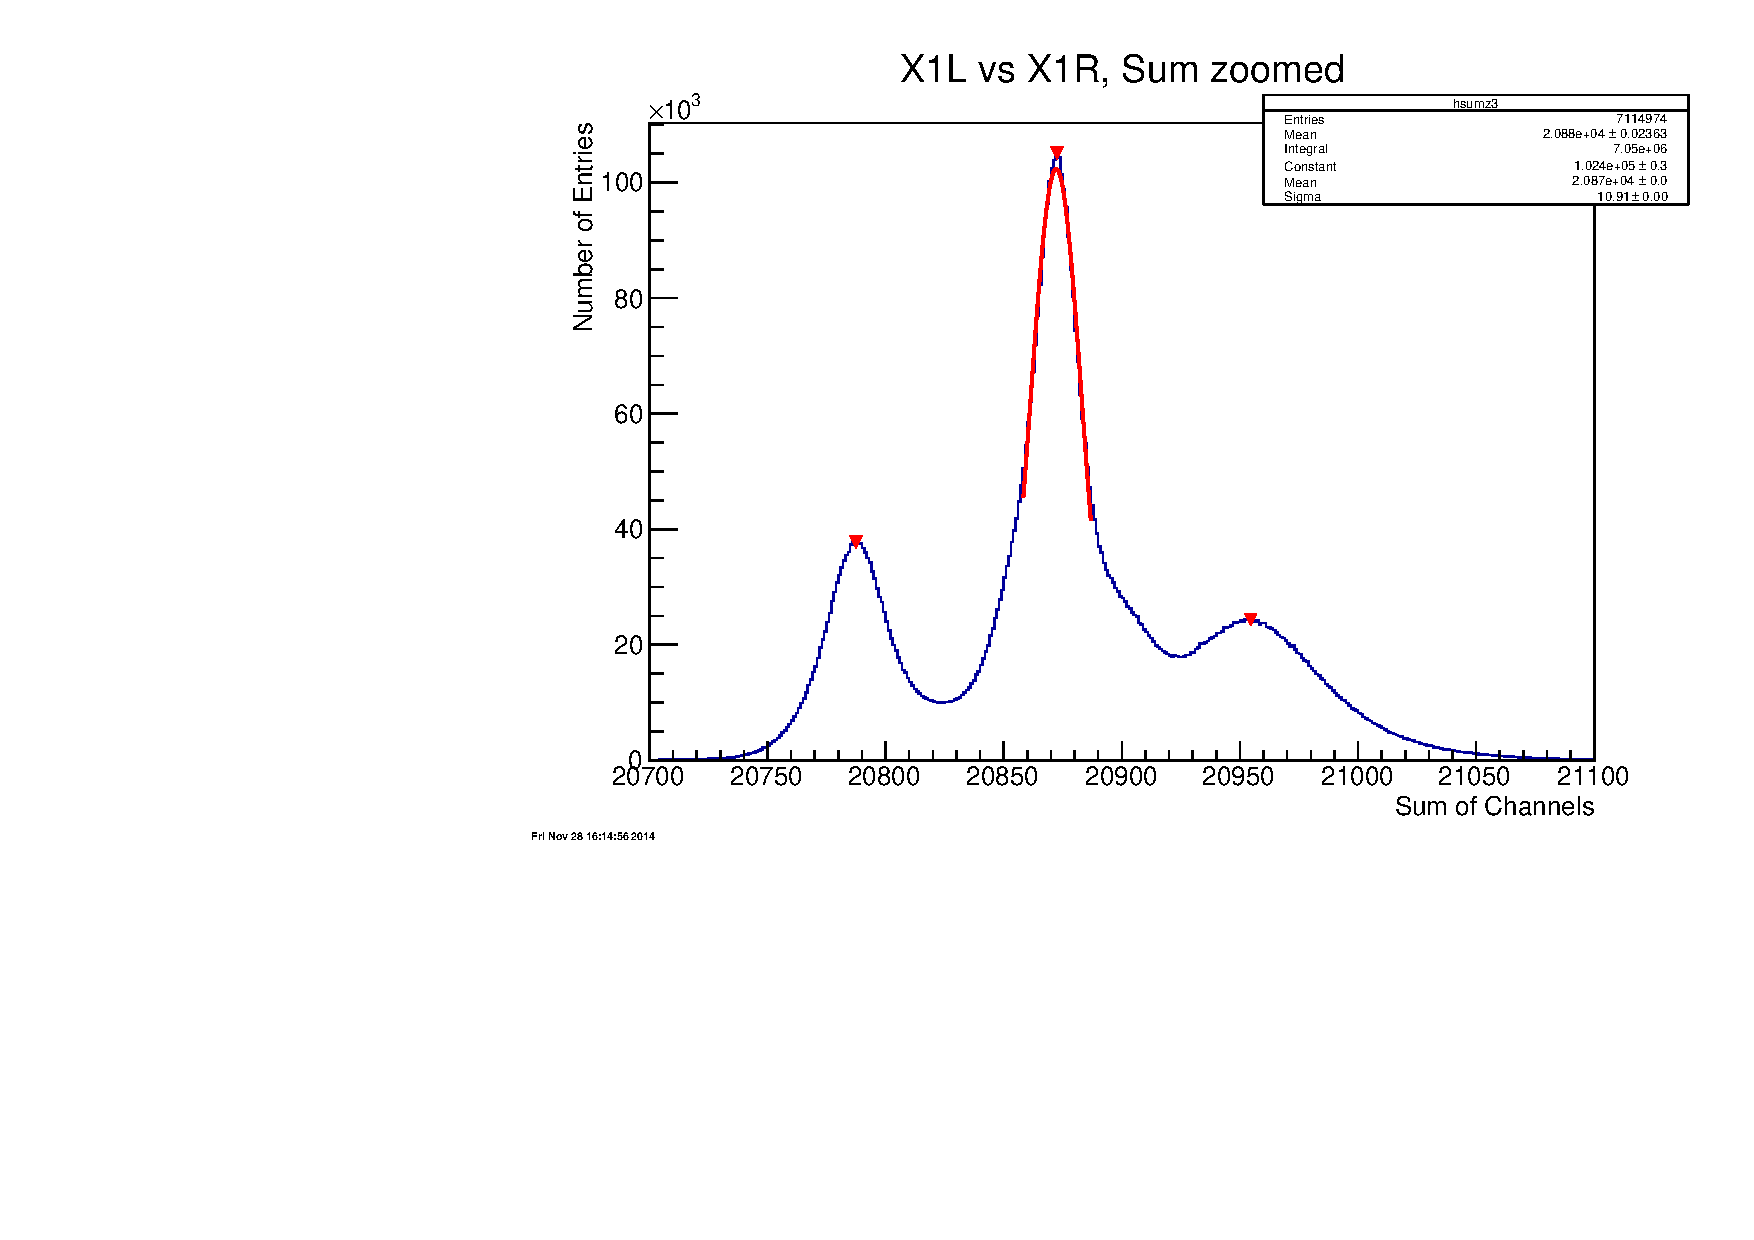
\includegraphics[width=0.48\textwidth, keepaspectratio]{run_430_hsumz3}\hspace{\fill}
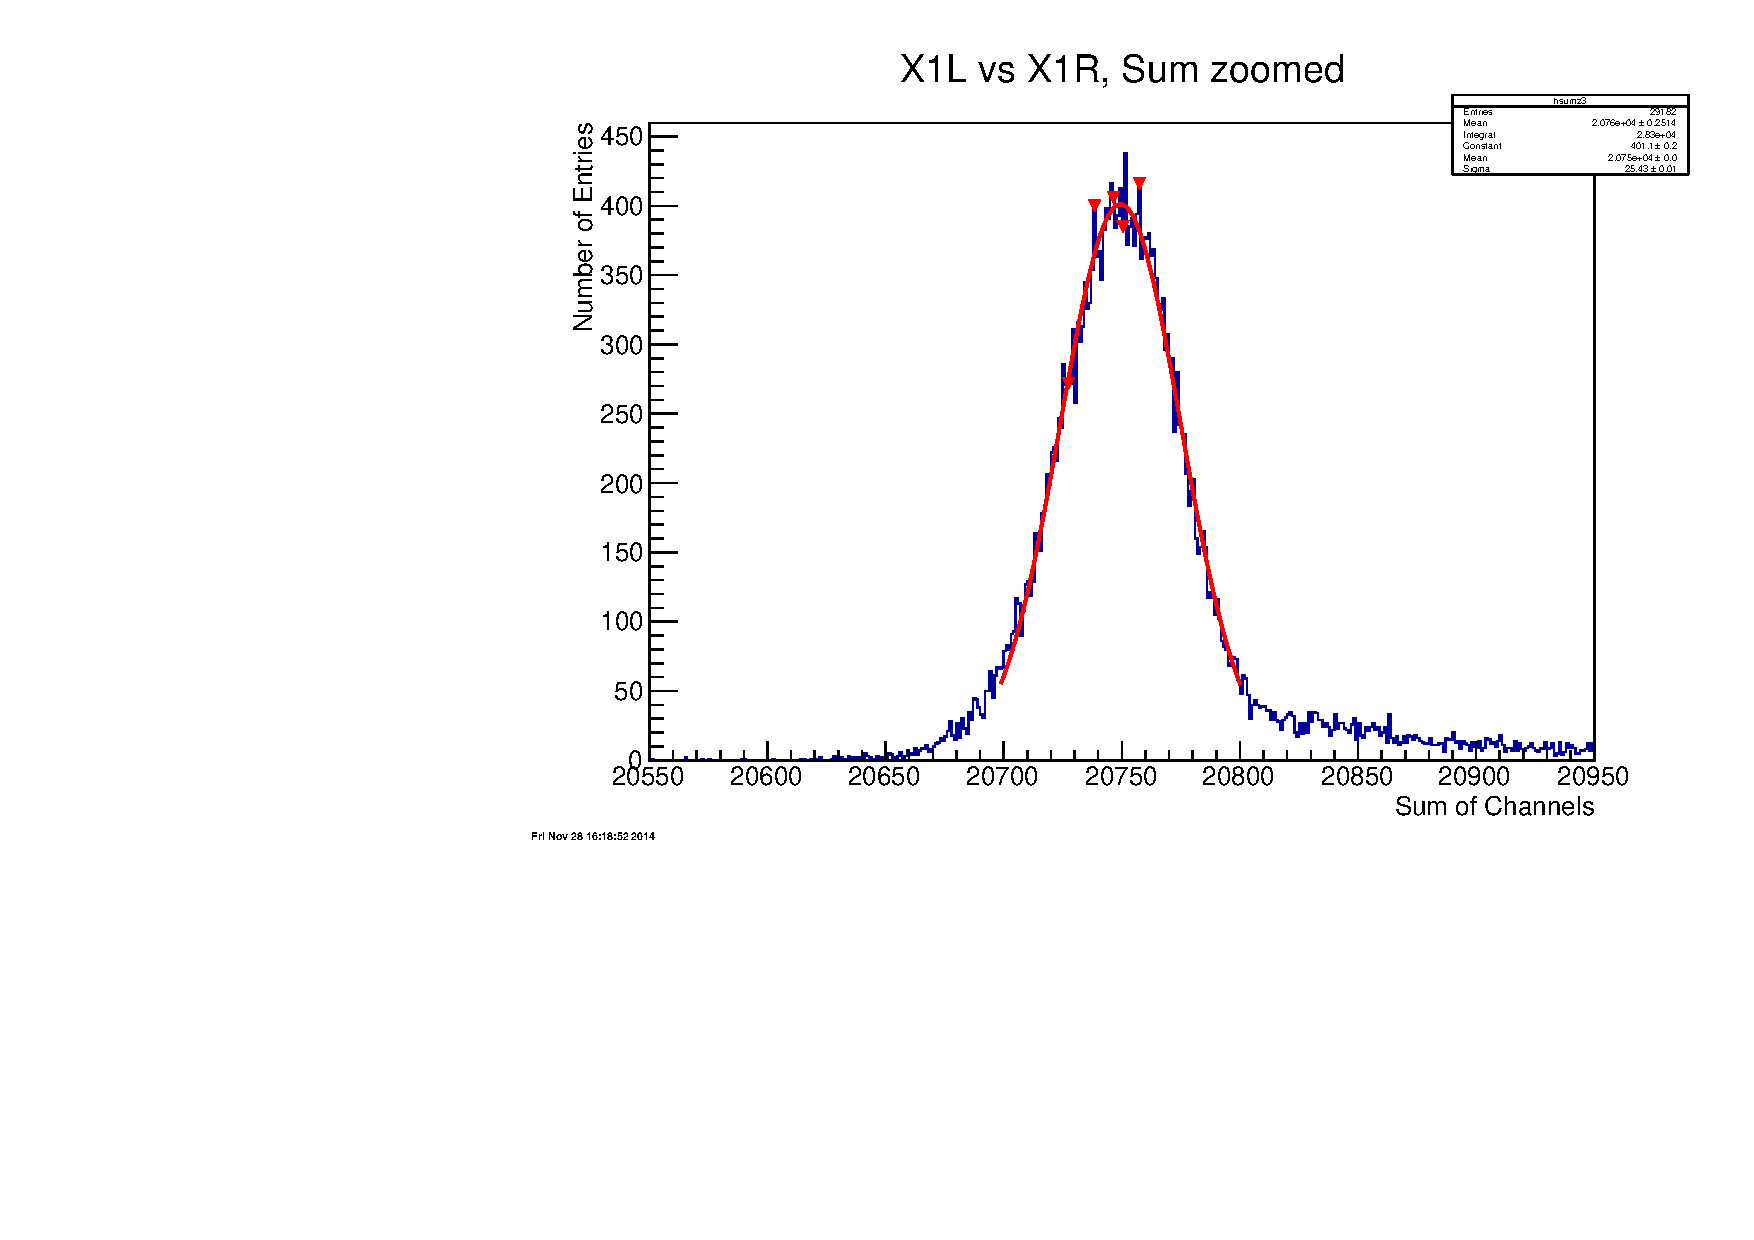
\includegraphics[width=0.48\textwidth, keepaspectratio]{run_480_hsumz3} \hspace{\fill}
\caption{Example cathode sum spectra for Run 430 (left) and Run 480 (right). In both figures, the sum of X1L and X1R is plotted over 400 channels. In Run 430, the sum spectra is divided into three peaks with 47\% of the data falling within $\pm 2 \sigma$ of the tallest peak. In Run 480, all of the data falls into a single peak with 83\% of the data falling within $\pm 2 \sigma$.}
\label{hsumz}
\end{figure}

Selecting the data based on this sharpness parameter is supported by examining the correlation between the difference in anode signals versus the sum of the various cathode channels. Such a plot is shown in Fig.~\ref{htsum}. All of the data with a sharpness parameter less than 2.8 correspond to data before Run 437. Referring to \S\ref{amp-settings}, one see that this corresponds to those runs which had a $10\times$ lower signal amplification at the input of the level discriminator and thus had higher peak-to-threshold ratio. Rejecting the data before Run 437 leaves 39 data runs.

\begin{figure}[ht]
\centering
\hspace{\fill}
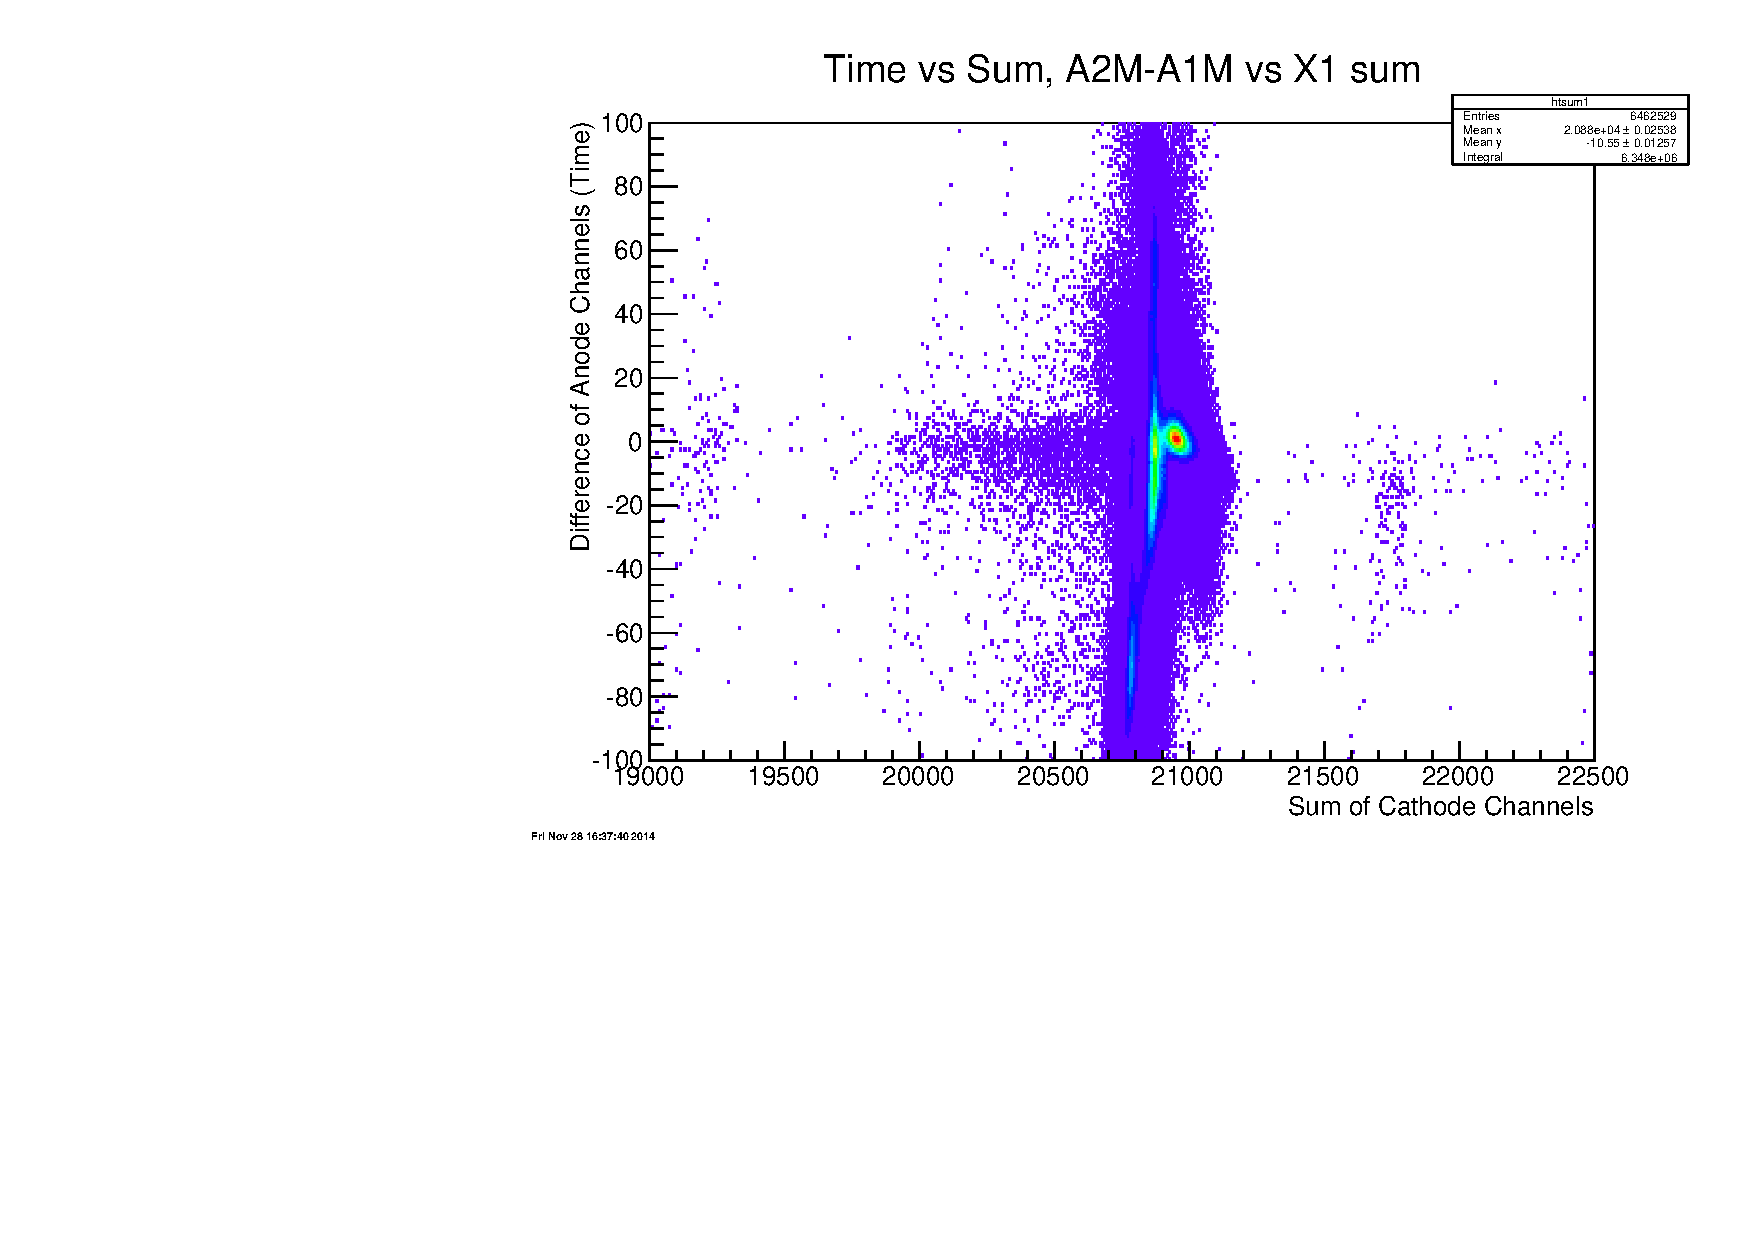
\includegraphics[width=0.48\textwidth, keepaspectratio]{run_430_htsum1}\hspace{\fill}
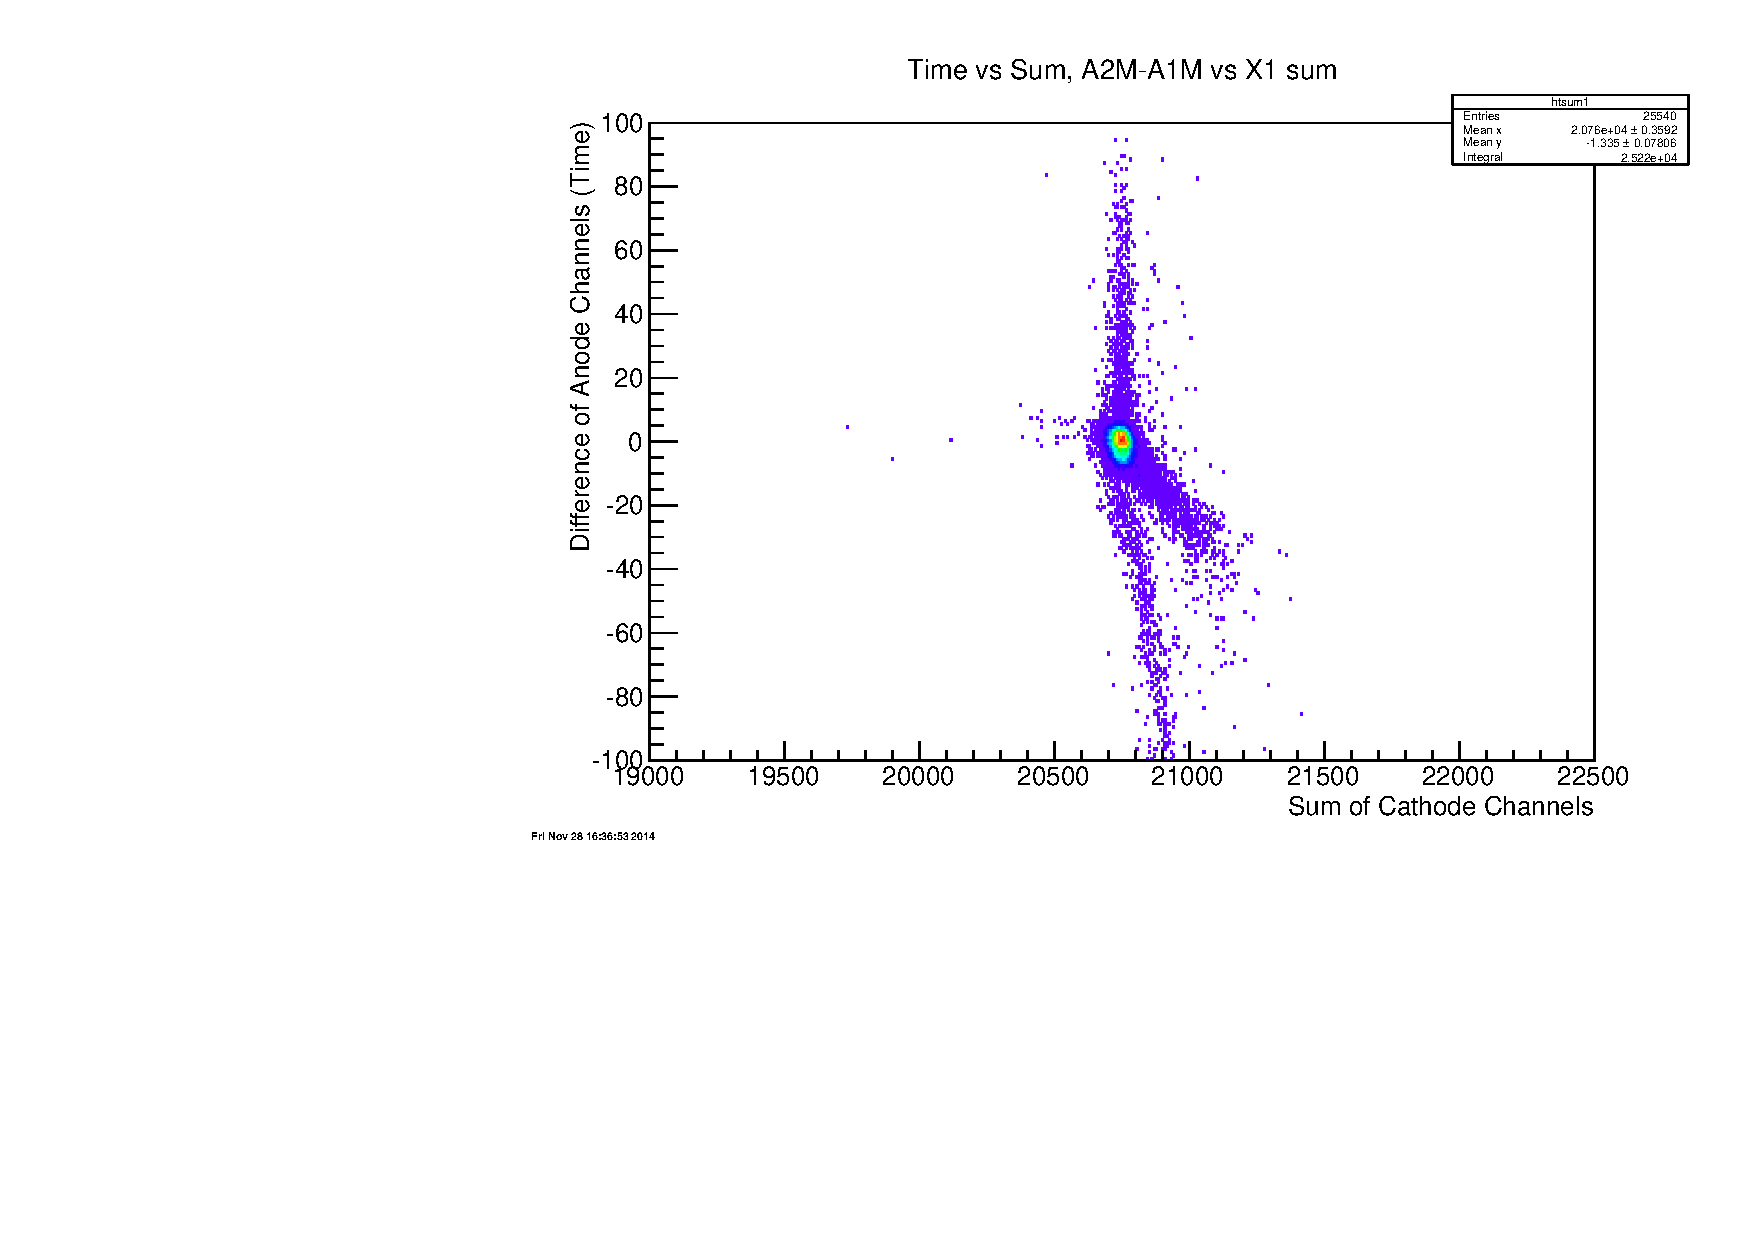
\includegraphics[width=0.48\textwidth, keepaspectratio]{run_480_htsum1} \hspace{\fill}
\caption{Example anode difference (time) vs cathode sum spectra for Run 430 (left) and Run 480 (right).}
\label{htsum}
\end{figure}

\subsubsection{Trigger rate}
Examining the trigger rate of the data runs further divides the data into two groups. The effective trigger rate was determined by measuring the number of anode coincidences and dividing by the duration of the run in seconds. 
\paragraph{2014 Test}
The data runs which used the digitizer 
%Most of the data runs 
had trigger rates less than 410 anode coincidences per second (74\,cps average). 
The data runs that did not use the digitizer %However, a number of the data runs 
had significantly higher trigger rates: over 2,000\,cps (7,400\,cps average). The data may be similarly divided based on the data rate.
%A number of the runs have data rates of 
Despite the higher event rate, the runs which did not use the digitizer have a lower data rate: 
less than 0.8\,MB/s (0.63\,MB/s average). 
The run which used the digitizer 
%Most of the runs 
have data rates greater than 3.4\,MB/s (10.1\,MB/s average). 

Excluding the non-digitizer runs, those runs with high trigger rates and low data rates, leaves 30 candidate data runs to assess the detector performance. The justification for this exclusion is explained in the next section. At the time of analysis, the  digitizer settings were not properly associated with their corresponding data runs. Therefore, it was unclear what the source of the varying data rates was.
\paragraph{2015 Test}
Most of the runs were without the digitizer enabled. The data rate for these runs was 89\,kB/s. With the digitizer enabled, the average data rate was 8.2\,MB/s. Unlike the 2014 test, the runs without the digitizer have excellent data. None of the pathological structures discussed in the previous section or the following section are present. This is likely due to proper triggering and optimized thresholds.

\subsubsection{Structure (2014 Test)}
The data from the high count rate (or low data rate) runs has some unusual structural features. For example, the results of the position calibration for detector 1 are shown in Fig.~\ref{overlay}. This data is from Run 430 and is generated with the following command.
\vsetroot
\begin{quote}
\begin{Verbatim}[firstnumber=0]
grantplot()
\end{Verbatim}
\end{quote}
\vsetnone
 The settings for this run are $P=3$\,Torr, $V_\textrm{c}=-75$\,V, $V_\textrm{a}=+420$\,V ($\Delta V=495$\,V). The beam current for this run was 4.24\,enA ($10\times$ attenuator). In the figure, the calculated projected positions of the mask features (red lines) and the positions of the Kapton shields (blue lines) have been overlaid with the data. The calculated positions of the calibration features are in good agreement with the data, indicated that the data has been properly calibrated. 

\begin{figure}
\centering
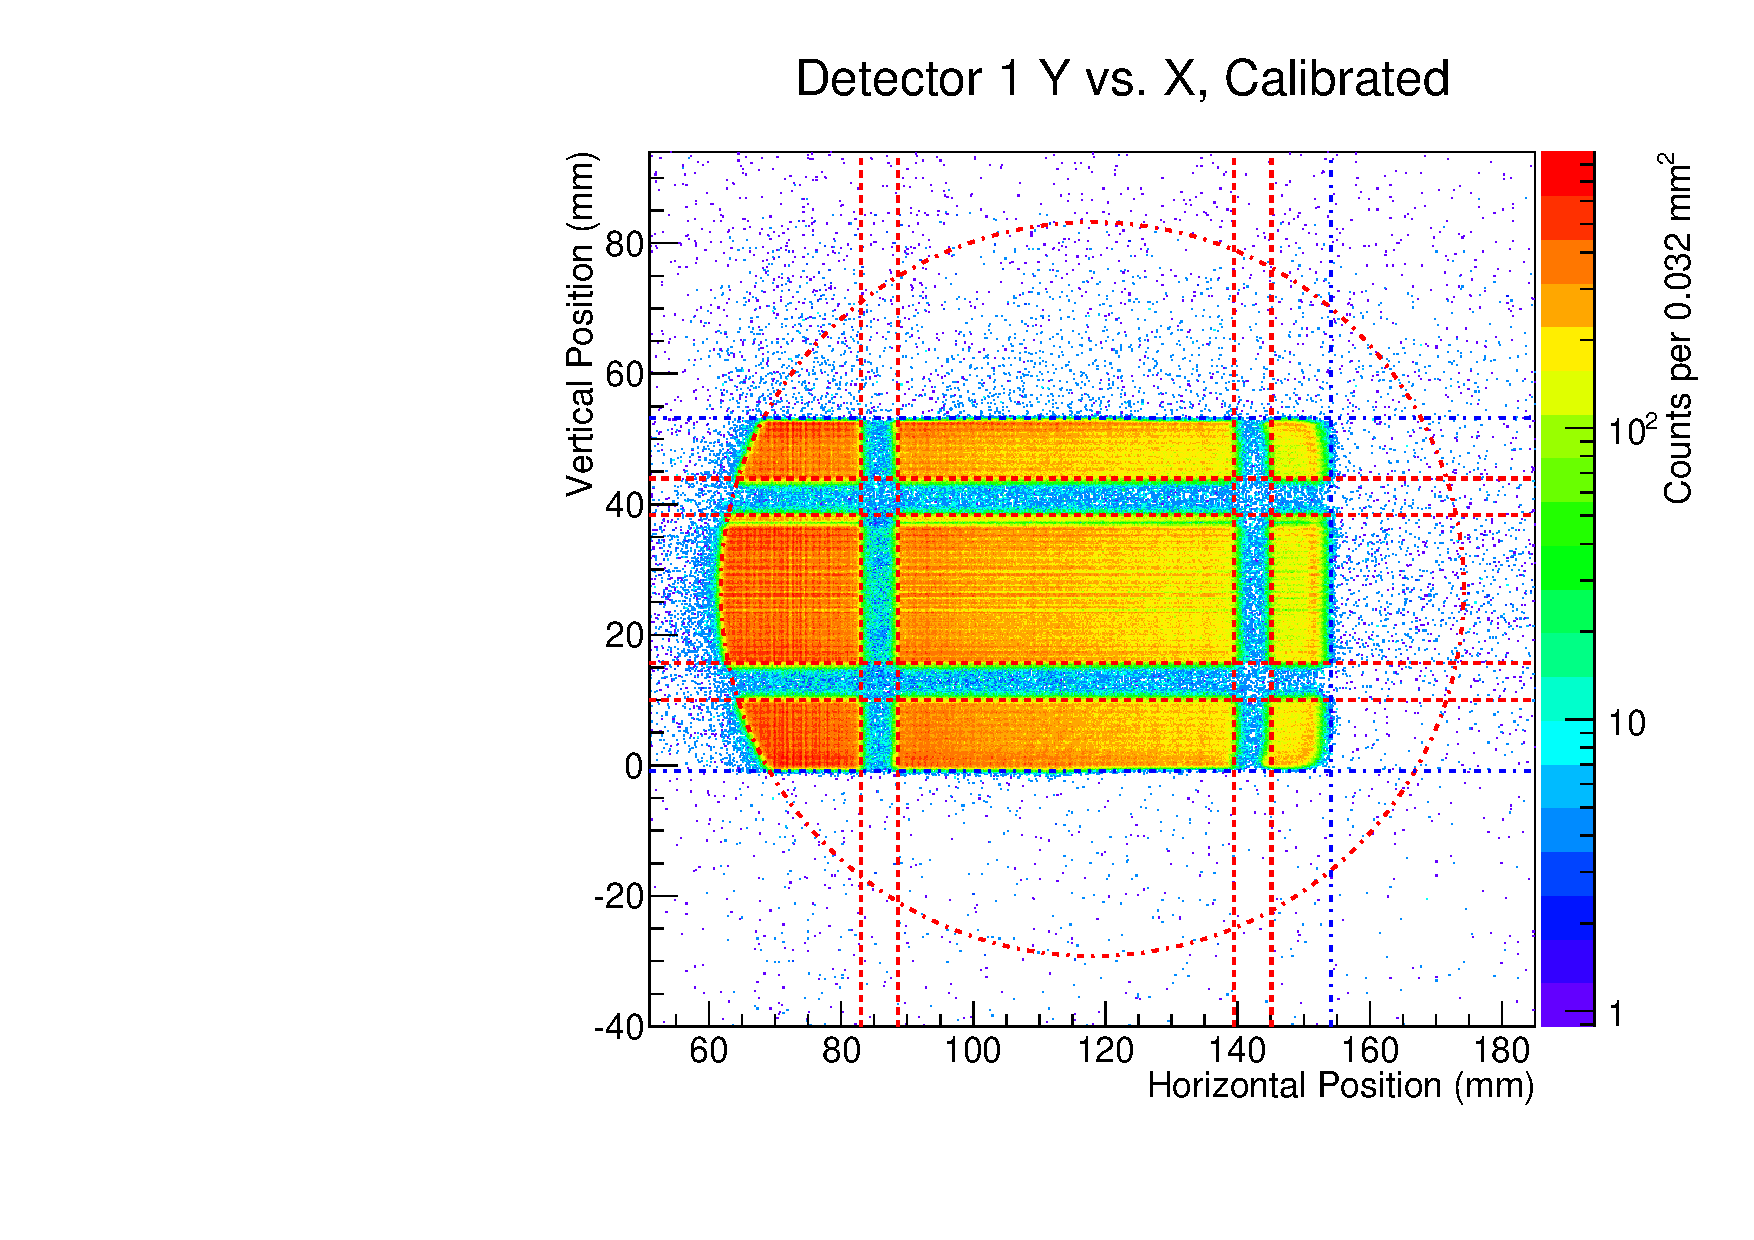
\includegraphics[width=\columnwidth,height=0.33\textheight,keepaspectratio]{run_430_hhitc0_overlay_c_log2z}%
\caption{Calibrated position spectrum for detector 1.  The calculated projections of the mask aperture (red dash-dotted line) and mask features (red dashed line) are plotted. The boundary of the fiducial area, corresponding to the location of the Kapton shields is also shown (blue dash-dotted line). Data from Run 430.}%
\label{overlay}%
\end{figure}

The wire grid of the cathodes is visibly resolved.  %demonstrating 
At first glance, this  would suggest that the detector resolution is $\lesssim 1$\,mm~FWHM. 
Fig.~\ref{peaks} shows a portion of the $y$-projection of Fig.~\ref{overlay}. The peaks have been fit and indicated with red arrows; the average gap between the peaks is 0.96\,mm. The width of the last peak is 0.47\,mm or 1.10\,mm~FWHM. This estimate of the resolution is borne out by the simulations as shown in Fig.~\ref{sim_comp2}. This figure is generated with the following macro in \texttt{load\_and\_plot.cc} which requires the PGAC simulation package \texttt{generator.cc}.
\vsetroot
\begin{quote}
\begin{Verbatim}[firstnumber=0]
resplot()
\end{Verbatim}
\end{quote}
\vsetnone
This behavior---that is, the resolution of the wire grid---is %typical of the detector and is
 visible at all pressures that were measured (2, 3, 4, and 6\,Torr). %It remains for the author to assess the dependence and variation of the detector resolution with the detector settings. 
The resolution of the \textit{anode} wires may be expected in the $y$-direction, however, inspection of Fig.~\ref{overlay} shows that resolution of a 1\,mm structure is present in both the $x$- and $y$-directions. The presence of the peaks in the $x$-direction makes this data suspect. This data is excluded by the trigger rate selection detailed in the previous section. This exclusion is justified by the trajectory analysis presented in the following section.
\begin{figure}
\centering
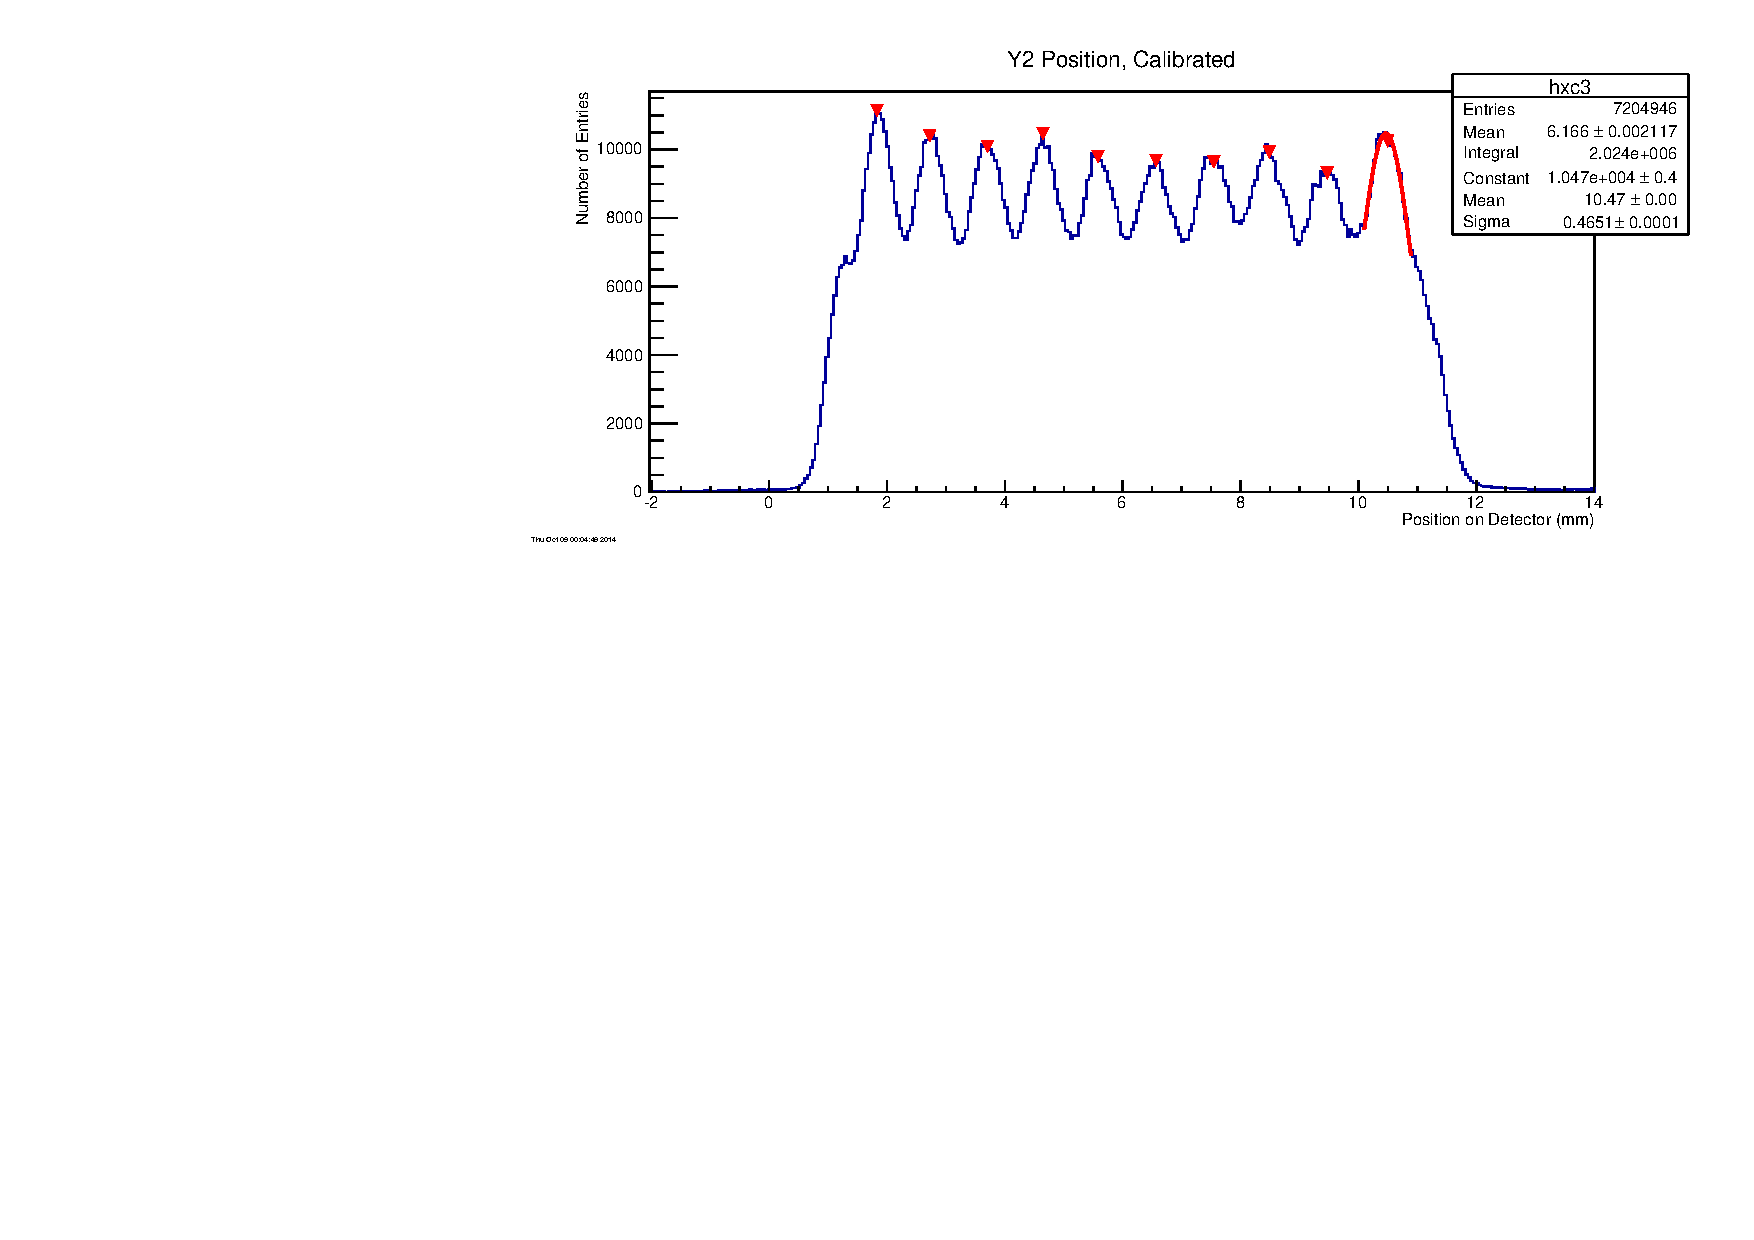
\includegraphics[width=\columnwidth,height=0.33\textheight,keepaspectratio]{run_430_hxc3}%
\caption{Example position spectrum showing the resolution of the cathode wires. The peaks have been identified and their positions are marked with red triangles. The last peak has been fit with a Gaussian for reference. This data is a portion of the $y$-projection ƒof Fig.~\ref{overlay}. Data from Run 430.}%
\label{peaks}%
\end{figure}

\begin{figure}%
\centering
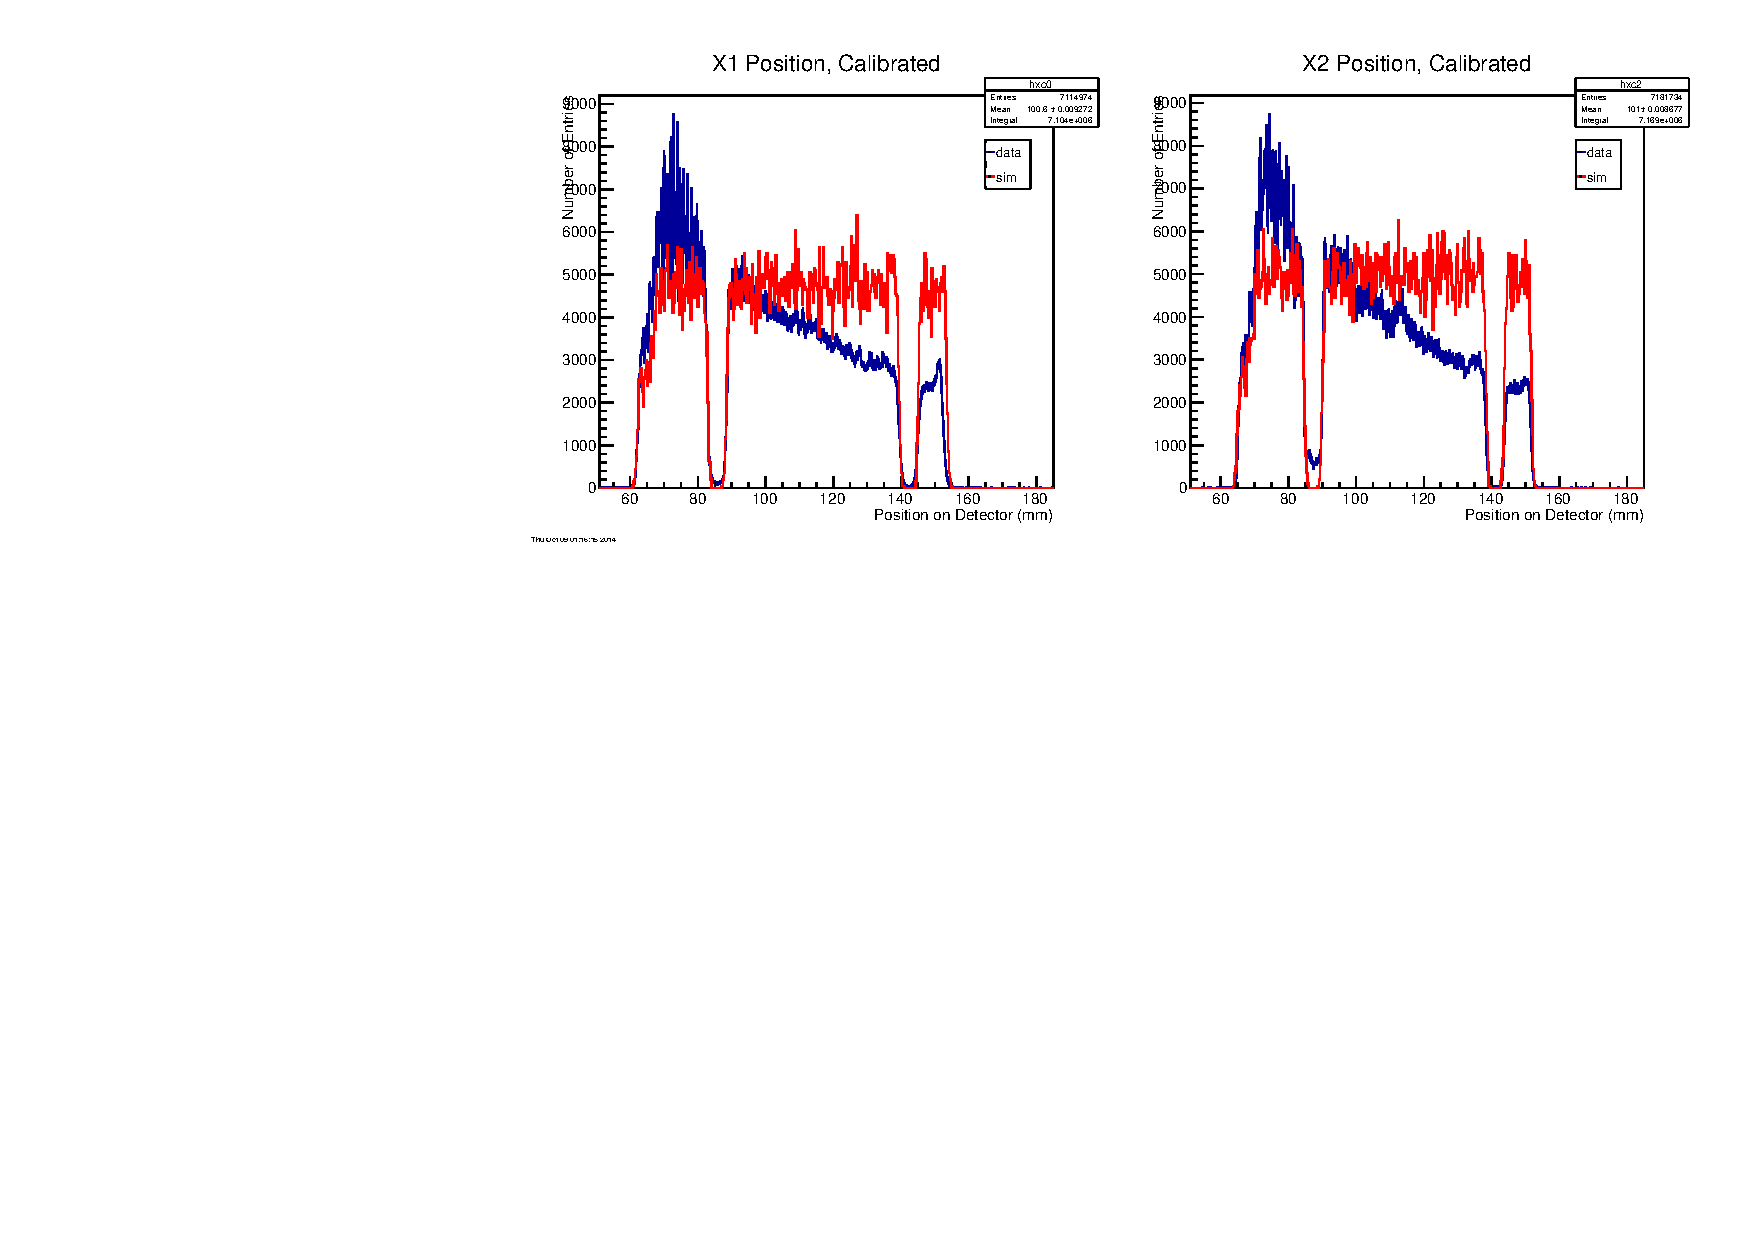
\includegraphics[width=\columnwidth,height=0.33\textheight,keepaspectratio]{run_430_compX}%
\caption{Simulated and measured $x$-position spectra of for each detector. The data (blue) have been fit with a simulated spectra using the following assumptions: a 1.43\,mm~FWHM beam spot centered at the origin and a detector resolution of 0.43\,mm (1.10\,mm~FWHM). Data from Run 430.}%
\label{sim_comp2}%
\end{figure}
\subsubsection{Trajectories}
Given the narrow trajectories incident to the detector---$\pm2.3^\circ$ in the $y$-direction and $-4.5^\circ$--3.0$^\circ$ in the $x$-direction---a strong correlation is expected between the position on each detector. Fig.~\ref{hxxc} shows the $x$-direction on detector 1 plotted as a function of the $x$-direction on detector 2; similarly for the $y$-direction. For Run 480 (bottom panel), the data form a single locus of points with a strong correlation between the detectors. The data from Run 430 (top panel) is characteristic of the high trigger rate runs. The expected locus of points is present, however, it is sitting on top of a background of variable gain and random correlation.

\begin{figure}
\centering
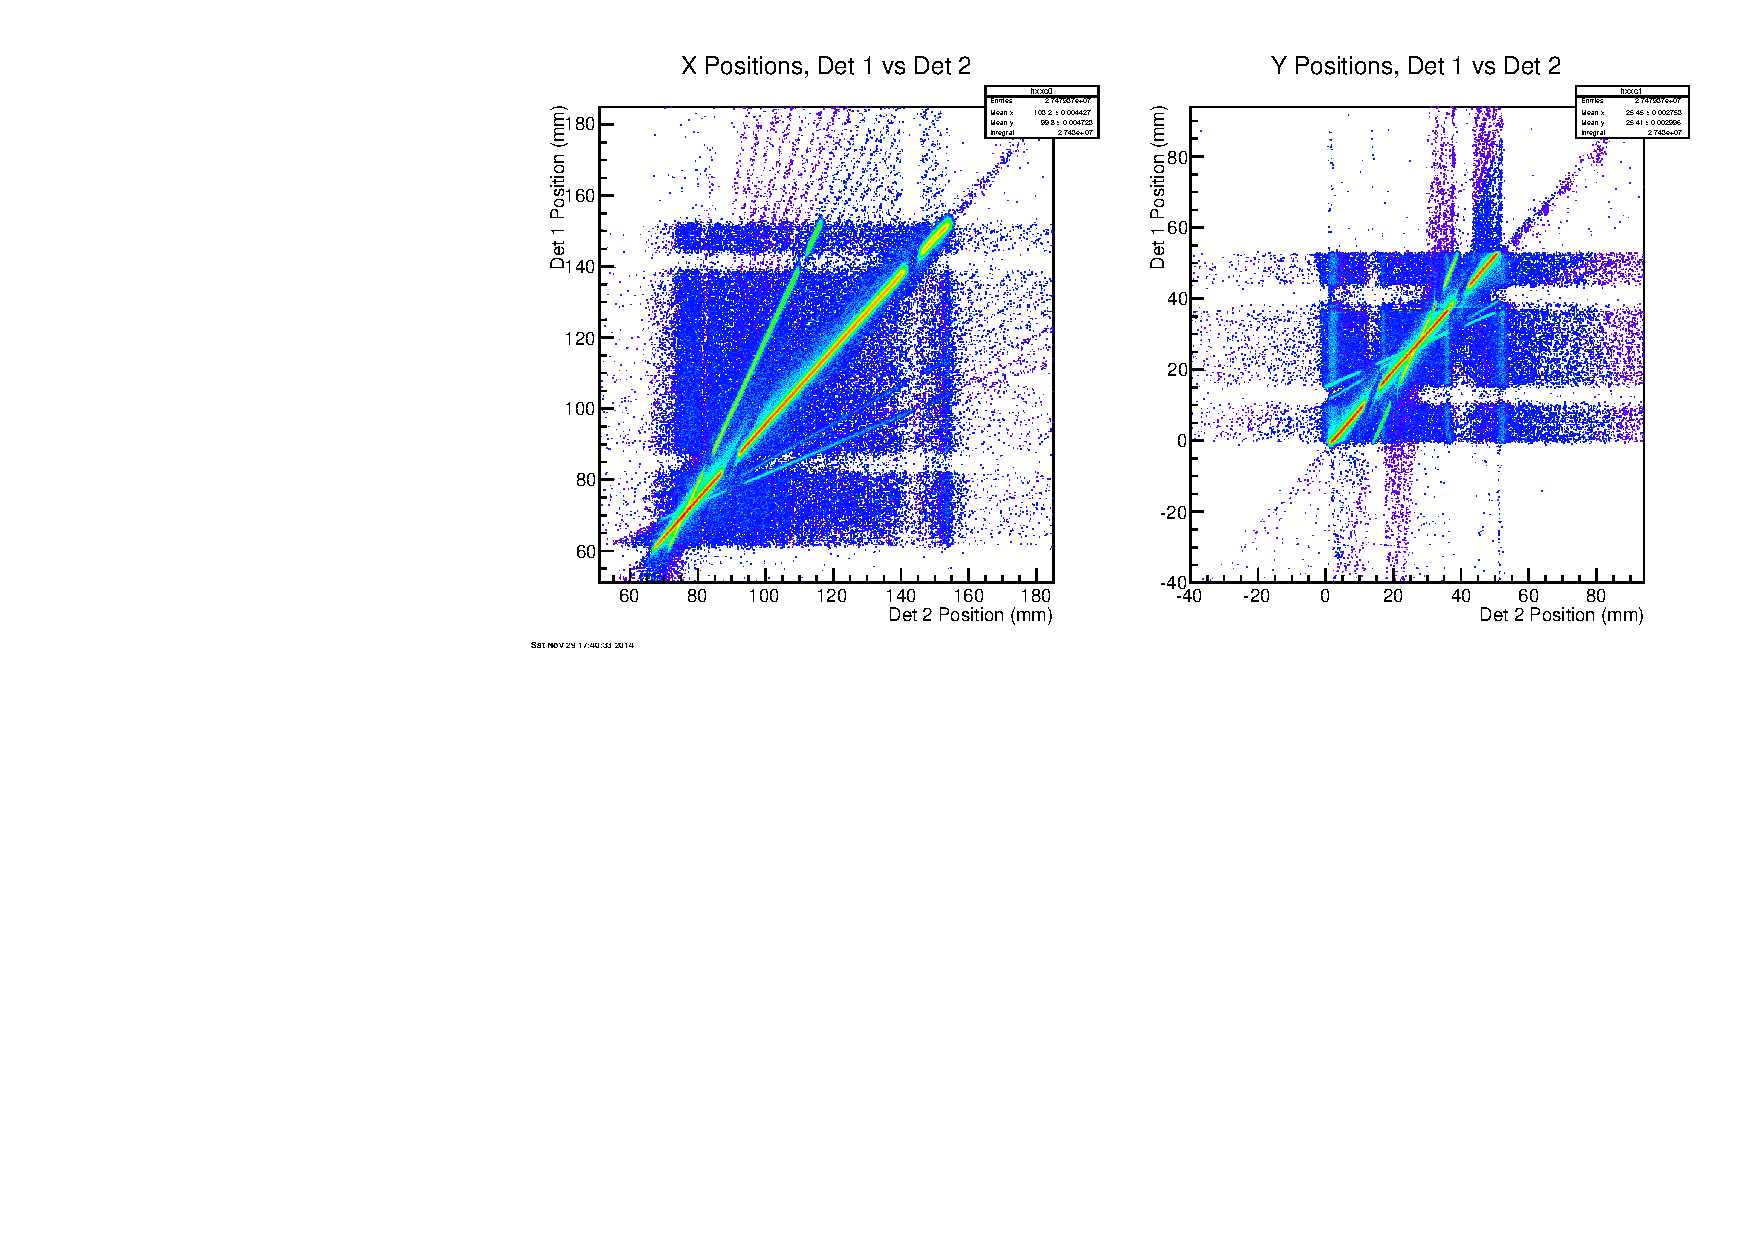
\includegraphics[width=\textwidth, height=0.33\textheight, keepaspectratio]{run_430_hxxc_2} \\
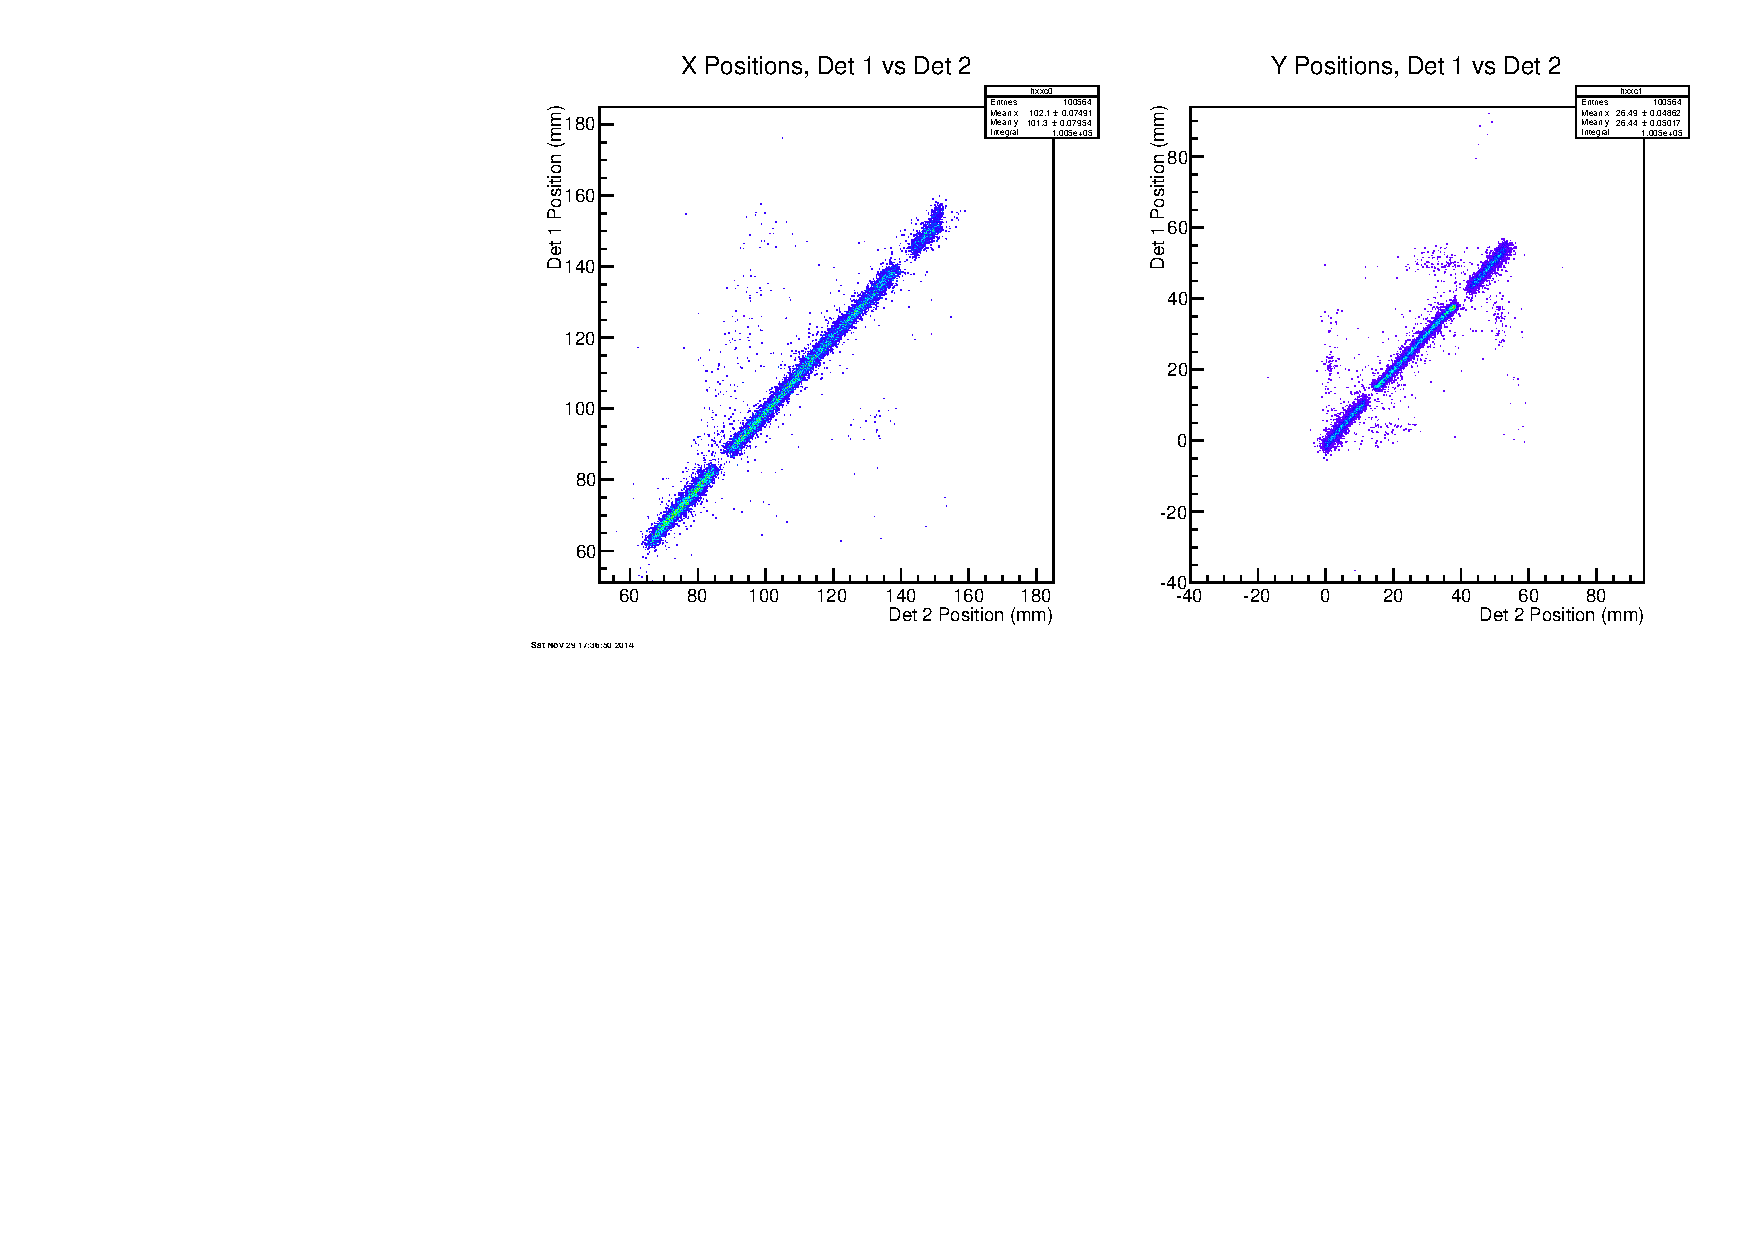
\includegraphics[width=\textwidth, height=0.33\textheight, keepaspectratio]{run_480_hxxc_2} 
\caption{Example  spectra for Run 430 (left) and Run 480 (right). }
\label{hxxc}
\end{figure}

The appearance of unphysical trajectories and random background are consistent with abnormal conditions such as sparking or triggering in the noise. Any of the data runs showing such pathological
Excluding all runs with unphysical behavior that are not otherwise excluded leaves 29 data runs for final analysis. 
\subsubsection{Summary}
The two most useful histograms for selecting data are the anode-time vs. cathode-sum plots (see Fig.~\ref{htsum} and the position correlation plots (see Fig.~\ref{hxxc}). Given an external time reference, the first example will still be useful in the final, single-detector setup.)
\subsection{Settings}
\label{settings_sec}
The detector and beam settings for the 29 data runs that were not excluded are shown in Table~\ref{run_list}. The summary of the 14 different combinations of detector and beam settings is shown in Table~\ref{settings}.
\begin{table}[ht!]
\centering
\begin{tabular}{crc..rccccr}
\hline
\multicolumn{2}{c}{Run} & \multicolumn{2}{c}{ADC} & \multicolumn{2}{c}{Beam} & & \multicolumn{3}{c}{Voltage}\\ \cline{1-2} \cline{5-6} \cline{8-10}
No. & Duration & On & \multicolumn{1}{c}{Sample} & \multicolumn{1}{c}{Current} & Atten. & $P$ & $V_\textrm{c}$ & $V_\textrm{a}$ & $\Delta V$ & Coinc.\\
\hline \hline
%438 & 598 & 0 & 1 & 5.62 & 10 & 3 & -74 & 411 & 485 & 32,159\\
%439 & 1154 & 1 & 5 & 5.62 & 10 & 3 & -74 & 411 & 485 & 16,836\\
%440 & 762 & 1 & 2.5 & 5.69 & 10 & 3 & -74 & 411 & 485 & 15,420\\
%444 & 397 & 1 & 1 & 5.69 & 10 & 4 & -80 & 430 & 510 & 24,941\\
%445 & 1,086 & 1 & 1 & 5.80 & 10 & 4 & -80 & 430 & 510 & 19,733\\
%446 & 538 & 1 & 1 & 5.89 & 10 & 4 & -80 & 430 & 510 & 38,811\\
%447 & 315 & 1 & 2.5 & 5.92 & 10 & 4 & -80 & 430 & 510 & 4,916\\
%449 & 294 & 0 & 5 & 5.99 & 10 & 6 & -90 & 470 & 560 & 8,095\\
%450 & 274 & 1 & 5 & 5.95 & 10 & 6 & -90 & 470 & 560 & 39,730\\
%451 & 244 & 1 & 5 & 5.86 & 10 & 6 & -90 & 480 & 570 & 28,987\\
%452 & 242 & 1 & 2.5 & 5.82 & 10 & 6 & -90 & 480 & 570 & 27,590\\
%454 & 273 & 0 & 1 & 5.75 & 10 & 6 & -90 & 450 & 540 & 38,737\\
%455 & 266 & 1 & 5 & 5.74 & 10 & 6 & -90 & 450 & 540 & 35,818\\
%456 & 690 & 1 & 2.5 & 5.75 & 10 & 6 & -90 & 450 & 540 & 25,818\\
%463 & 242 & 0 & 1 & 4.30 & 10 & 2 & -80 & 400 & 480 & 33,211\\
%465 & 321 & 0 & 1 & 0.52 & 10 & 2 & -80 & 390 & 470 & 22,758\\
%467 & 176 & 1 & 1 & 0.54 & 10 & 2 & -80 & 395 & 475 & 22,083\\
%468 & 327 & 1 & 1 & 0.52 & 10 & 2 & -80 & 395 & 475 & 11,334\\
%470 & 307 & 1 & 1 & 5.60 & 10 & 3 & -75 & 410 & 485 & 5,817\\
%471 & 378 & 1 & 1 & 5.66 & 10 & 3 & -75 & 410 & 485 & 40,467\\
%472 & 285 & 1 & 1 & 5.63 & 10 & 3 & -75 & 390 & 465 & 31,042\\
%473 & 361 & 1 & 1 & 5.59 & 10 & 3 & -75 & 375 & 450 & 20,511\\
%474 & 318 & 1 & 1 & 5.50 & 10 & 4 & -80 & 430 & 510 & 8,141\\
%475 & 429 & 1 & 1 & 5.55 & 10 & 4 & -80 & 430 & 510 & 12,470\\
%476 & 392 & 1 & 1 & 0.51 & 120 & 4 & -80 & 430 & 510 & 29,756\\
%477 & 315 & 1 & 1 & 34.00 & 1 & 4 & -80 & 410 & 490 & 2,679\\
%478 & 72 & 1 & 1 & 0.65 & 120 & 4 & -80 & 445 & 525 & 29,251\\
%479 & 595 & 1 & 1 & 0.65 & 120 & 4 & -80 & 445 & 525 & 2,073\\
%480 & 805 & 1 & 1 & 0.64 & 120 & 3 & -80 & 435 & 515 & 28,465\\
438 & 598 & 1 & 5 & 5.62 & 10 & 3 & -74 & 411 & 485 & 32,159\\
439 & 1154 & 1 & 2.5 & 5.62 & 10 & 3 & -74 & 411 & 485 & 16,836\\
440 & 762 & 1 & 1 & 5.69 & 10 & 3 & -74 & 411 & 485 & 15,420\\
444 & 397 & 1 & 1 & 5.69 & 10 & 4 & -80 & 430 & 510 & 24,941\\
445 & 1086 & 1 & 1 & 5.80 & 10 & 4 & -80 & 430 & 510 & 19,733\\
446 & 538 & 1 & 2.5 & 5.89 & 10 & 4 & -80 & 430 & 510 & 38,811\\
447 & 315 & 1 & 5 & 5.92 & 10 & 4 & -80 & 430 & 510 & 4,916\\
449 & 294 & 1 & 5 & 5.99 & 10 & 6 & -90 & 470 & 560 & 8,095\\
450 & 274 & 1 & 5 & 5.95 & 10 & 6 & -90 & 470 & 560 & 39,730\\
451 & 244 & 1 & 2.5 & 5.86 & 10 & 6 & -90 & 480 & 570 & 28,987\\
452 & 242 & 1 & 1 & 5.82 & 10 & 6 & -90 & 480 & 570 & 27,590\\
454 & 273 & 1 & 5 & 5.75 & 10 & 6 & -90 & 450 & 540 & 38,737\\
455 & 266 & 1 & 2.5 & 5.74 & 10 & 6 & -90 & 450 & 540 & 35,818\\
456 & 690 & 1 & 1 & 5.75 & 10 & 6 & -90 & 450 & 540 & 25,818\\ \hline
463 & 242 & 1 & 1 & 4.30 & 10 & 2 & -80 & 400 & 480 & 33,211\\
465 & 321 & 1 & 1 & 0.52 & 10 & 2 & -80 & 390 & 470 & 22,758\\
467 & 176 & 1 & 1 & 0.54 & 10 & 2 & -80 & 395 & 475 & 22,083\\
468 & 327 & 1 & 1 & 0.52 & 10 & 2 & -80 & 395 & 475 & 11,334\\
470 & 307 & 1 & 1 & 5.60 & 10 & 3 & -75 & 410 & 485 & 5,817\\
471 & 378 & 1 & 1 & 5.66 & 10 & 3 & -75 & 410 & 485 & 40,467\\
472 & 285 & 1 & 1 & 5.63 & 10 & 3 & -75 & 390 & 465 & 31,042\\
473 & 361 & 1 & 1 & 5.59 & 10 & 3 & -75 & 375 & 450 & 20,511\\
474 & 318 & 1 & 1 & 5.50 & 10 & 4 & -80 & 430 & 510 & 8,141\\
475 & 429 & 1 & 1 & 5.55 & 10 & 4 & -80 & 430 & 510 & 12,470\\
476 & 392 & 1 & 1 & 0.51 & 120 & 4 & -80 & 430 & 510 & 29,756\\
477 & 315 & 1 & 1 & 34.00 & 1 & 4 & -80 & 410 & 490 & 2,679\\
478 & 72 & 1 & 1 & 0.65 & 120 & 4 & -80 & 445 & 525 & 29,251\\
479 & 595 & 1 & 1 & 0.65 & 120 & 4 & -80 & 445 & 525 & 2,073\\
480 & 805 & 1 & 1 & 0.64 & 120 & 3 & -80 & 435 & 515 & 28,465\\
\hline
\end{tabular}
\caption{Detector, acquisition, and beam settings from April 2014 for the 29 runs which are not excluded. Given are the run number and the run duration (in seconds). The settings for digitizer, here referred to as the ADC, are given: the enable state and the sample rate (in GS/s). The nominal beam current is given (in enA) and the associated setting of the IOS attenuator is given. Note that for a number of the 2\,Torr runs, the beam current fell off by a factor of $10\times$. The detector settings are given next: pressure (in Torr) and voltage (in V). Finally the number of anode coincidences is given. The horizontal line indicates a new day of testing.}
\label{run_list}
\end{table}

\begin{table}[ht!]
\centering
\begin{tabular}{crc..rccccr}
\hline
\multicolumn{2}{c}{Run} & \multicolumn{2}{c}{ADC} & \multicolumn{2}{c}{Beam} & & \multicolumn{3}{c}{Voltage}\\ \cline{1-2} \cline{5-6} \cline{8-10}
No. & Duration & On & \multicolumn{1}{c}{Sample} & \multicolumn{1}{c}{Current} & Atten. & $P$ & $V_\textrm{c}$ & $V_\textrm{a}$ & $\Delta V$ & Coinc.\\
\hline \hline
%584 & 633 & 0 & 0 & 9.00 &  & 3 & -75 & 410.5 & 485.5 & 0\\
%586 & 294 & 0 & 0 & 8.50 &  & 3 & -75 & 411 & 486 & 0\\ \hline
%587 & 1813 & 0 & 0 & 13.00 &  & 3 & -75 & 410 & 485 & 0\\
%588 & 1221 & 1 & 1 & 12.89 &  & 3 & -75 & 410 & 485 & 0\\
%589 & 2113 & 0 & 0 & 13.00 &  & 3 & -75 & 410 & 485 & 0\\
%590 & 500 & 0 & 0 & 1.20 &  & 3 & -75 & 410 & 485 & 0\\
%592 & 425 & 0 & 0 & 12.95 &  & 3 & -75 & 410 & 485 & 0\\
%593 & 1143 & 0 & 0 & 12.89 &  & 3 & -79 & 410.5 & 489.5 & 0\\
%594 & 1214 & 0 & 0 & 12.71 &  & 2 & -78 & 397 & 475 & 0\\
%595 & 620 & 1 & 1 & 12.65 &  & 2 & -78 & 397 & 475 & 0\\
%596 & 126 & 0 & 0 & 12.60 &  & 2 & -78 & 397 & 475 & 0\\
%597 & 199 & 1 & 2.5 & 12.24 &  & 2 & -78 & 397 & 475 & 0\\
%598 & 152 & 1 & 5 & 12.48 &  & 2 & -78 & 397 & 475 & 0\\
%599 & 103 & 1 & 1 & 12.60 &  & 2 & -78 & 397 & 475 & 0\\
%600 & 153 & 0 & 0 & 12.60 &  & 2 & -78 & 397 & 475 & 0\\
%602 & 1677 & 0 & 0 & 12.13 &  & 2 & -78 & 397 & 475 & 0\\ \hline
%603 & 2247 & 0 & 0 & 20.00 &  & 4 & -82 & 429 & 511 & 0\\
%604 & 345 & 1 & 1 & 20.55 &  & 4 & -82 & 429 & 511 & 0\\
%606 & 1013 & 0 & 0 & 22.42 &  & 4 & -82 & 429 & 511 & 0\\
%607 & 402 & 1 & 1 & 22.42 &  & 4 & -82 & 429 & 511 & 0\\
%608 & 517 & 0 & 0 & 370.00 &  & 4 & -82 & 429 & 511 & 0\\
%609 & 318 & 1 & 1 & 387.34 &  & 4 & -82 & 429 & 511 & 0\\
%610 & 1203 & 1 & 1 & 1.89 &  & 4 & -82 & 429 & 511 & 0\\
%611 & 821 & 1 & 1 & 1.72 &  & 4 & -82 & 429 & 511 & 0\\
584 & 633 & 0 & 0 & 9.00 & 1 & 3 & -75 & 410.5 & 485.5 & 323,593\\
586 & 294 & 0 & 0 & 8.50 & 1 & 3 & -75 & 411 & 486 & 127,047\\ \hline
587 & 1813 & 0 & 0 & 13.00 & 2 & 3 & -75 & 410 & 485 & 1,171,411\\
588 & 1221 & 1 & 1 & 12.89 & 2 & 3 & -75 & 410 & 485 & 9,705\\
589 & 2113 & 0 & 0 & 13.00 & 2 & 3 & -75 & 410 & 485 & 1,381,064\\
590 & 500 & 0 & 0 & 1.20 & 10 & 3 & -75 & 410 & 485 & 28,330\\
592 & 425 & 0 & 0 & 12.95 & 2 & 3 & -75 & 410 & 485 & 273,850\\
593 & 1143 & 0 & 0 & 12.89 & 2 & 3 & -79 & 410.5 & 489.5 & 737,678\\
594 & 1214 & 0 & 0 & 12.71 & 2 & 2 & -78 & 397 & 475 & 779,734\\
595 & 620 & 1 & 1 & 12.65 & 2 & 2 & -78 & 397 & 475 & 10,466\\
596 & 126 & 0 & 0 & 12.60 & 2 & 2 & -78 & 397 & 475 & 79,535\\
597 & 199 & 1 & 2.5 & 12.24 & 2 & 2 & -78 & 397 & 475 & 970\\
598 & 152 & 1 & 5 & 12.48 & 2 & 2 & -78 & 397 & 475 & 22,823\\
599 & 103 & 1 & 1 & 12.60 & 2 & 2 & -78 & 397 & 475 & 1,698\\
600 & 153 & 0 & 0 & 12.60 & 2 & 2 & -78 & 397 & 475 & 94,607\\
%602 & 1677 & 0 & 0 & 12.13 & 2 & 2 & -78 & 397 & 475 & 136,172\\
 \hline
603 & 2247 & 0 & 0 & 20.00 & 3 & 4 & -82 & 429 & 511 & 2,148,241\\
604 & 345 & 1 & 1 & 20.55 & 3 & 4 & -82 & 429 & 511 & 15,532\\
606 & 1013 & 0 & 0 & 22.42 & 3 & 4 & -82 & 429 & 511 & 1,011,153\\
607 & 402 & 1 & 1 & 22.42 & 3 & 4 & -82 & 429 & 511 & 2,746\\
608 & 517 & 0 & 0 & 370.00 & 0.1 & 4 & -82 & 429 & 511 & 3,404,786\\
609 & 318 & 1 & 1 & 387.34 & 0.1 & 4 & -82 & 429 & 511 & 8,507\\
610 & 1203 & 1 & 1 & 1.89 & 10 & 4 & -82 & 429 & 511 & 2,904\\
611 & 821 & 1 & 1 & 1.72 & 10 & 4 & -82 & 429 & 511 & 23,338\\


\hline
\end{tabular}
\caption{Detector, acquisition, and beam settings for the 24 data runs from the April 2015 in-beam tests. Given are the run number and the run duration (in seconds). The settings for digitizer, here referred to as the ADC, are given: the enable state and the sample rate (in GS/s). The nominal beam current is given (in enA) and the associated setting of the IOS attenuator is given.
% Note that for a number of the 2\,Torr runs, the beam current fell off by a factor of $10\times$.
 The detector settings are given next: pressure (in Torr) and voltage (in V). Finally the number of anode coincidences is given. Data from each of the three days are separated by horizontal lines.}
\label{run_list_2}
\end{table}

\begin{table}[ht!]
\centering
\begin{tabular}{cccc.rrr}
\hline
& \multicolumn{3}{c}{Voltage} & \multicolumn{2}{c}{Beam}\\ \cline{2-4} 
$P$& $V_\textrm{c}$ & $V_\textrm{a}$ & $\Delta V$ & \multicolumn{1}{c}{Current} & Atten. & \multicolumn{1}{c}{Duration} & \multicolumn{1}{c}{Coinc.}\\
\hline \hline
2 & -80 & 390 & 470 & 0.52 & 10 & 321 & 22,758\\
2 & -80 & 395 & 475 & 0.53 & 10 & 503 & 33,417\\
2 & -80 & 400 & 480 & 4.30 & 10 & 242 & 33,211\\ \hline
3 & -75 & 375 & 450 & 5.59 & 10 & 361 & 20,511\\
3 & -75 & 390 & 465 & 5.63 & 10 & 285 & 31,042\\
3 & -74 & 411 & 485 & 5.64 & 10 & 3,199 & 110,699\\
3 & -80 & 435 & 515 & 0.64 & 120 & 805 & 28,465\\ \hline
4 & -80 & 410 & 490 & 34.00 & 1 & 315 & 2,679\\
4 & -80 & 430 & 510 & 5.73 & 10 & 3,083 & 109,012\\
4 & -80 & 430 & 510 & 0.51 & 120 & 392 & 29,756\\
4 & -80 & 445 & 525 & 0.65 & 120 & 667 & 31,324\\ \hline
6 & -90 & 450 & 540 & 5.75 & 10 & 1,229 & 100,373\\
6 & -90 & 470 & 560 & 5.97 & 10 & 568 & 47,825\\
6 & -90 & 480 & 570 & 5.84 & 10 & 486 & 56,577\\
\hline
\end{tabular}
\caption{Summary of the different detector and beam settings used for the 2014 test. For each detector setting, the average beam current is given (in enA) and the associated IOS attenuator setting. Similarly, the total duration of the runs (in seconds) and the total anode coincidences are given.}
\label{settings}
\end{table}
\subsubsection{Detector}
In the 2014 tests, four different pressures were tested. At each pressure, the voltage was varied in order %The goal of the experiment was 
to determine the maximum stable operating voltage. The maximum stable operating voltage was determined by the highest voltage the detector was able to maintain for 5--10\,minutes without sparking. If a spark occurred within that interval, the bias voltage was reduced and the timing procedure was restarted. Such as with the $P=2$\,Torr data shown in Table~\ref{run_list}, depending on the step size used to reduce the voltage, the voltage may then be further increased. For each pressure, at least three different voltages were tested which yielded adequate data. 

Table~\ref{max_V} shows the results of the maximum stable operating pressure tests. For these tests, the IOS attenuator setting remained constant at $10\times$ and the nominal beam current was 5.70\,enA. The relationship between the detector pressure $P$ and the maximum stable voltage difference $\Delta V_\textrm{max}$ is linear and described by the following equation.
\begin{equation}
\Delta V_\textrm{max}=16.86 P%\,\frac{\textrm{V}}{\textrm{torr}}
 +  439.3%\,\textrm{V}
\label{eq:vmax}
\end{equation}
Here the voltage difference $\Delta V_\textrm{max}$ is given in V and the pressure $P$ is given in V/torr. %$\dfrac{\textrm{V}}{\textrm{torr}}$
The average ratio between the maximum stable voltage difference and the maximum stable anode voltage is 83.9\%.
\begin{equation}
V_\textrm{a}=0.839 \Delta V_\textrm{max}
\label{eq:vamax}
\end{equation}
Here both values are given in volts. The calculated maximum stable operating voltages are also %results of these two equations are 
given in Table~\ref{max_V}.

\begin{table}[!ht]
\centering
\begin{tabular}{cccc|ccc}
\hline
& \multicolumn{3}{c|}{Measured}  %\cline{2-4} 
& \multicolumn{3}{c}{Calculated} \\ \cline{2-7} 
$P$& $V_\textrm{c}$ & $V_\textrm{a}$ & $\Delta V$ & $V_\textrm{c}$ & $V_\textrm{a}$ &$\Delta V_\textrm{calc}$ \\
\hline \hline
%2 & -80 & 395 & 475&473.0\\
%3 & -75 & 410 & 485&489.9\\
%4 & -80 & 430 & 510&506.7\\
%6 & -90 & 450 & 540&540.4\\
1.5 & --- &--- & --- & 389.6 & -75.0 & 464.6\\
2.0 & -80 &395 & 475 & 396.6 & -76.4 & 473.0\\
2.5 & --- &--- & --- & 403.7 & -77.7 & 481.4\\
3.0 & -75 &410 & 485 & 410.8 & -79.1 & 489.9\\
3.5 & --- &--- & --- & 417.9 & -80.4 & 498.3\\
4.0 & -80 &430 & 510 & 424.9 & -81.8 & 506.7\\
4.5 & --- &--- & --- & 432.0 & -83.2 & 515.1\\
5.5 & --- &--- & --- & 446.1 & -85.9 & 532.0\\
6.0 & -90 &450 & 540 & 453.2 & -87.2 & 540.4\\
\hline
\end{tabular}
\caption{Maximum stable voltage settings for each pressure determined from the 2014 tests. The beam current was nominally 5.70\,enA for these tests. Where available, the measured maximum stable voltages are given. The maximum statable voltage $\Delta V_\textrm{calc}$ %is related to the 
is %can be
 calculated for %an arbitrary
 each pressure using by Eq.~\ref{eq:vmax}.  The calculated ratio between $V_\textrm{a}$  and $\Delta V_\textrm{calc}$ is given by Eq.~\ref{eq:vamax}.}
\label{max_V}
\end{table}
\subsubsection{Beam}
A beam rate test was carried out at $P=4$\,Torr. Three different beam attenuator settings were used. As expected, the lower the beam current, the higher the voltage difference the detector was able to support without sparking. In the final moments of the experiment, the detector was tested at $P=3$\,Torr with the low beam current setting. Again, a higher maximum stable voltage was possible. Note that during the $P=2$\,Torr runs, the beam current dropped off by a factor of $10\times$. This was not due to a change in attenuator setting.
\subsubsection{Acquisition}
The digitizer (ADC) was operated at three different sampling frequencies: 1.0, 2.5, and 5.0\,GS/s; corresponding to timing resolutions of 1.00\,ns, 400\,ps, and 200\,ps, respectively. The $P=3$\,Torr data at $\Delta V=485$\,V includes all four possible ADC settings---that is, enabled and disabled, and all three sample rates. \marnote{check!}The various ADC settings had no correlation with the resolution of the TDC data.%\pangram{40}

\subsection{Position Resolution}
The width of the sum of cathode signals gives an upper limit on the position resolution. Assessing the position resolution in this way has the benefit of utilizing a simple and reliable fitting algorithm---that is, a least squares fit of a Gaussian function.

\subsubsection{Relative Width}
The relative widths corresponding to the positions remained effectively constant throughout the variety of detector settings. In the 2014 test, Detector 1 had slightly better resolution than detector 2: on average, the width of X2 was 108\% wider than that of X1; and, on average, the width of Y2 was 106\% wider than X1. In the 2015 test, Detector 2 had slightly better position resolution. 
In both tests, the position resolution was better in the $y$-direction. The average width of the $x$-position peaks was 146\%--177\% that of the average width of the $y$-position peaks. Putting all of the position peak widths in terms of the width of Y1:\\% X1 144\%, Y1 100\%, X2 156\%, Y2 106\%.
\begin{center}
\begin{tabular}{ccc}
 \hline 
Pos.& \multicolumn{2}{c}{Ratio} \\ \cline{2-3} 
&2014 & 2015\\\hline\hline
 X1 & 144\%&161\%\\
 Y1 & 100\%&100\%\\
 X2 & 156\%&155\%\\
 Y2 & 106\%&79\%\\\hline
 

\end{tabular}
\end{center}

\subsubsection{Voltage Dependence}
At each of the pressure settings of $P=2$, 3, and 6\,Torr, three different voltage settings were tested at the same beam current which provided nominal data.
For $P=2$ and 3\,Torr  %each pressure,
the data were fit with a quadratic function to determine 
%In each case, the maximum stable voltage was determined to be the lowest voltage given.
the minimum peak width. % was calculated for each pressure. 
For each quantity a global minimization was performed %found
 with the condition that the quadratic coefficient be positive and the discriminant be negative to ensure that a valid minimum was determined.
Table~\ref{pos_res_fit} shows the results of that calculation.

The variation in peak width with applied voltage for the $P=2$\,Torr data was relatively flat, with only X1 showing a clear 
minimum within the rage of voltages tested. Also, because of the falloff in beam current, the results from the $P=2$\,Torr data may be inconclusive. 
The variation in peak width for $P=3$\,Torr is show in Fig.~\ref{min_fit}. Each of the positions had a minimum within the range of measured voltages.
For $P=2$ and 3\,Torr, the results of the fit are in good agreement with the maximum stable operating voltage shown in Table~\ref{max_V}. This independent agreement suggests that the optimal operating voltage is the same as the maximum stable operating voltage.

For the data at $P=4$, 6\,Torr the maximum stable voltage was %determined to be 
the same as the lowest voltage tested. For $P=4$\,Torr, only one point was available for the $10\times$ attenuator setting. For $P=6$\,Torr, the peak width decreased approaching $\Delta V=540$\,V. However, no data for $\Delta V < 540$\,V was measured, so a representative fit could not be made. For $P=4$ and 6\,Torr, the ``Average'' value given in Table~\ref{pos_res_fit} is the result of Eq.~\ref{eq:vmax}.


\begin{figure}
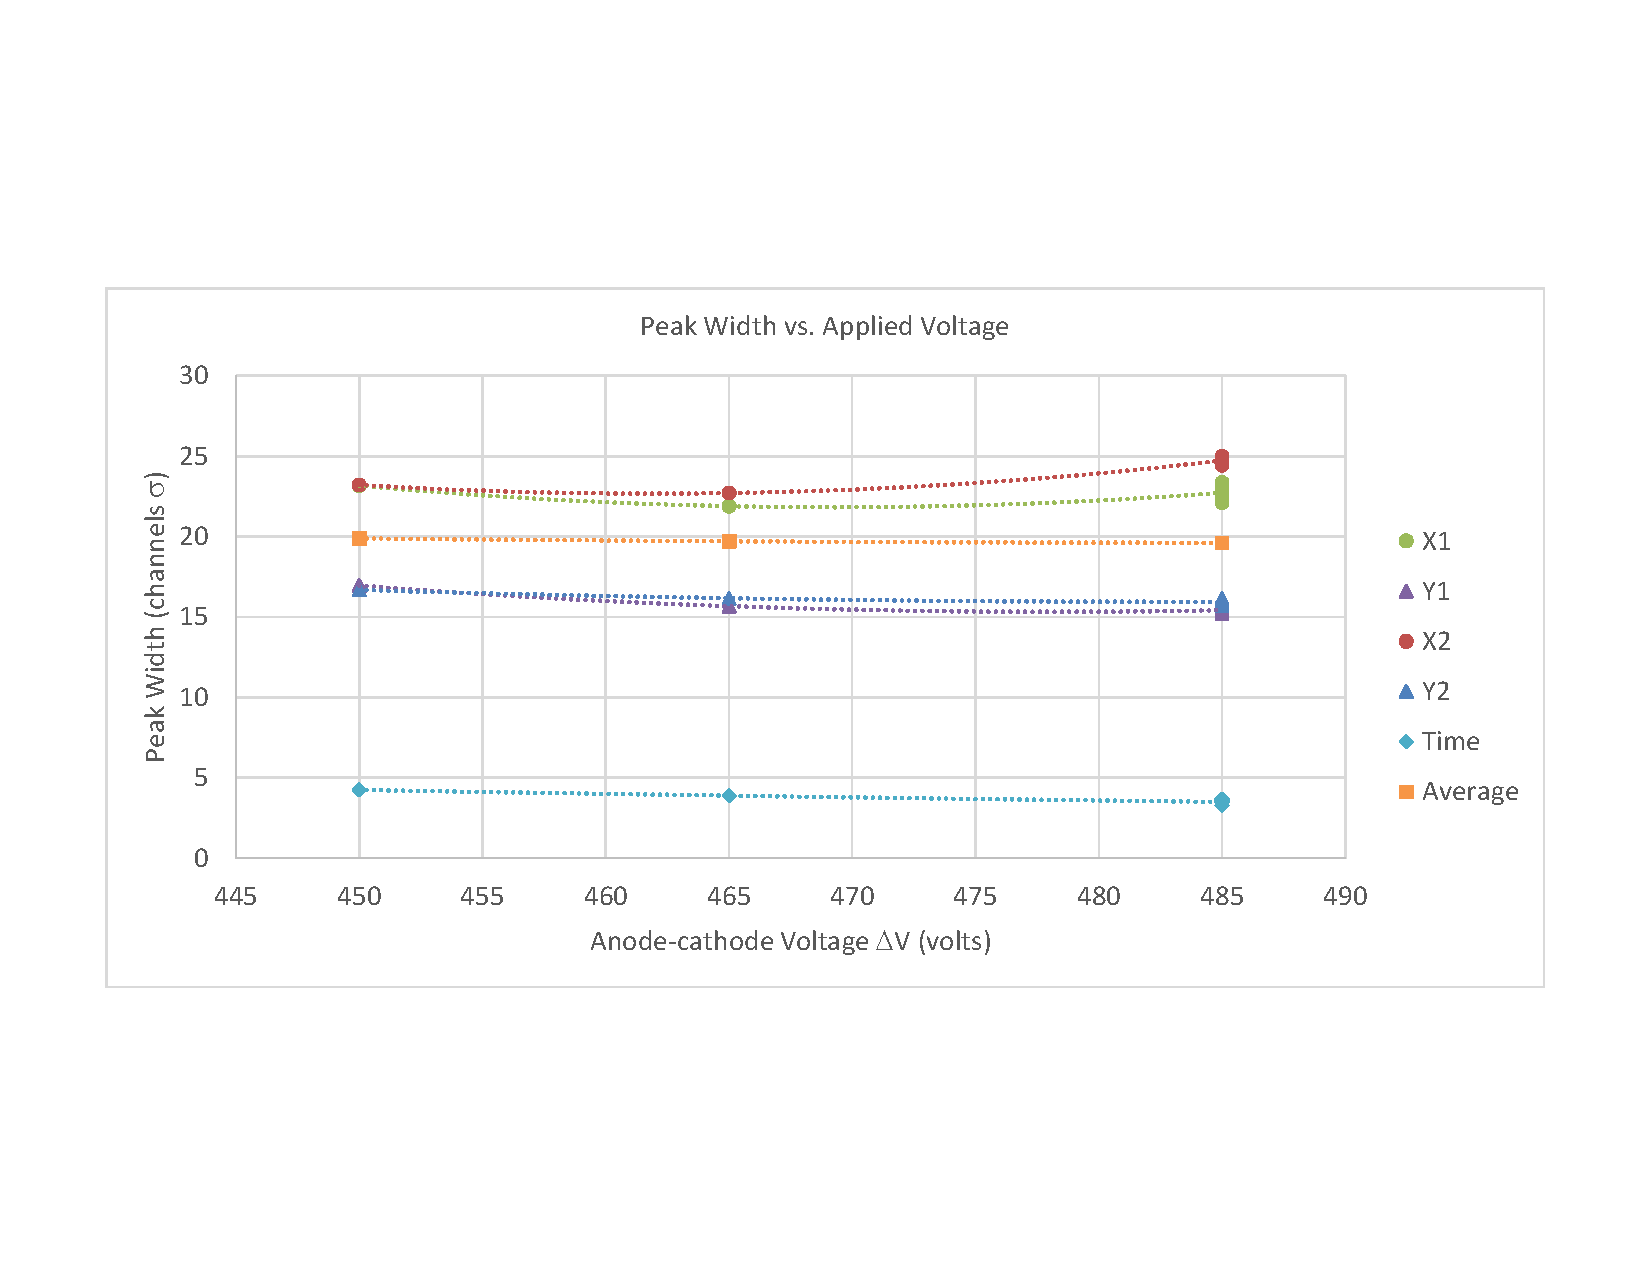
\includegraphics[width=\columnwidth]{PGAC_test_run_list_av_6}%
\caption{Peak width variance with applied voltage %$\Delta V$
 at $P=3$\,Torr. The beam current was nominally 5.70\,enA for all runs. The detector was tested at three different voltages from 450--485V. For each position, the variation of the width of the position peaks was fit with a quadratic function.  The average minimum of these fits was 488.4\,V. The average of the positions is also plotted.}%
\label{min_fit}%
\end{figure}

\begin{table}[ht!]
\centering
\begin{tabular}{cccccccc|c}
\hline
& \multicolumn{2}{c}{Voltage} & \multicolumn{6}{c}{Fit Minima}\\ \cline{4-9}
Pressure & Min & Max & Time & X1 & Y1 & X2 & Y2 & Average\\ \hline \hline
2 & 470 & 480 & 475.0 & 476.0 & 475.3 & 474.0 & 474.9 & 475.0\\
3  & 450 & 485 & --- & 470.4 & 493.5 & 471.5 & 483.4 & 488.4\\
4  & 510 & 510 & --- & --- & --- & --- & --- & 506.7\\
6  & 540 & 570 & --- & --- & --- & --- & --- & 540.4\\
\hline
\end{tabular}
\caption{Calculated optimal voltage for each pressure setting. At each pressure, the maximum and minimum voltage that was tested is given. The beam attenuator setting was the same for all of these runs, with a nominal beam current of 5.70\,enA. Each data set for $P=2$, 3\,Torr was fit with a quadratic function. Where applicable, the minimum of each fit and the average of the minima are given. For $P=4$, 6\,Torr the ``Average'' minimum is given by Eq.~\ref{eq:vmax}. The data for $P=3$\,Torr is shown in Fig.~\ref{min_fit}. }
\label{pos_res_fit}
\end{table}

\subsubsection{Pressure Dependence}
Fig.~\ref{pressure_width} shows the variation of the various peak widths as a function of pressure. For all data sets, the voltage difference is set to the maximum stable operating voltage and the nominal beam current is 5.70\,enA.
 Table~\ref{av_peak_vs_pressure} shows the average peak width for the time and positions at the maximum stable operating voltage at each pressure. Recall the time peak is the difference of the anode signals; and the position peaks are the sum of the cathode signals. Each data set for each position has been fit with a quadratic function.


\begin{figure}
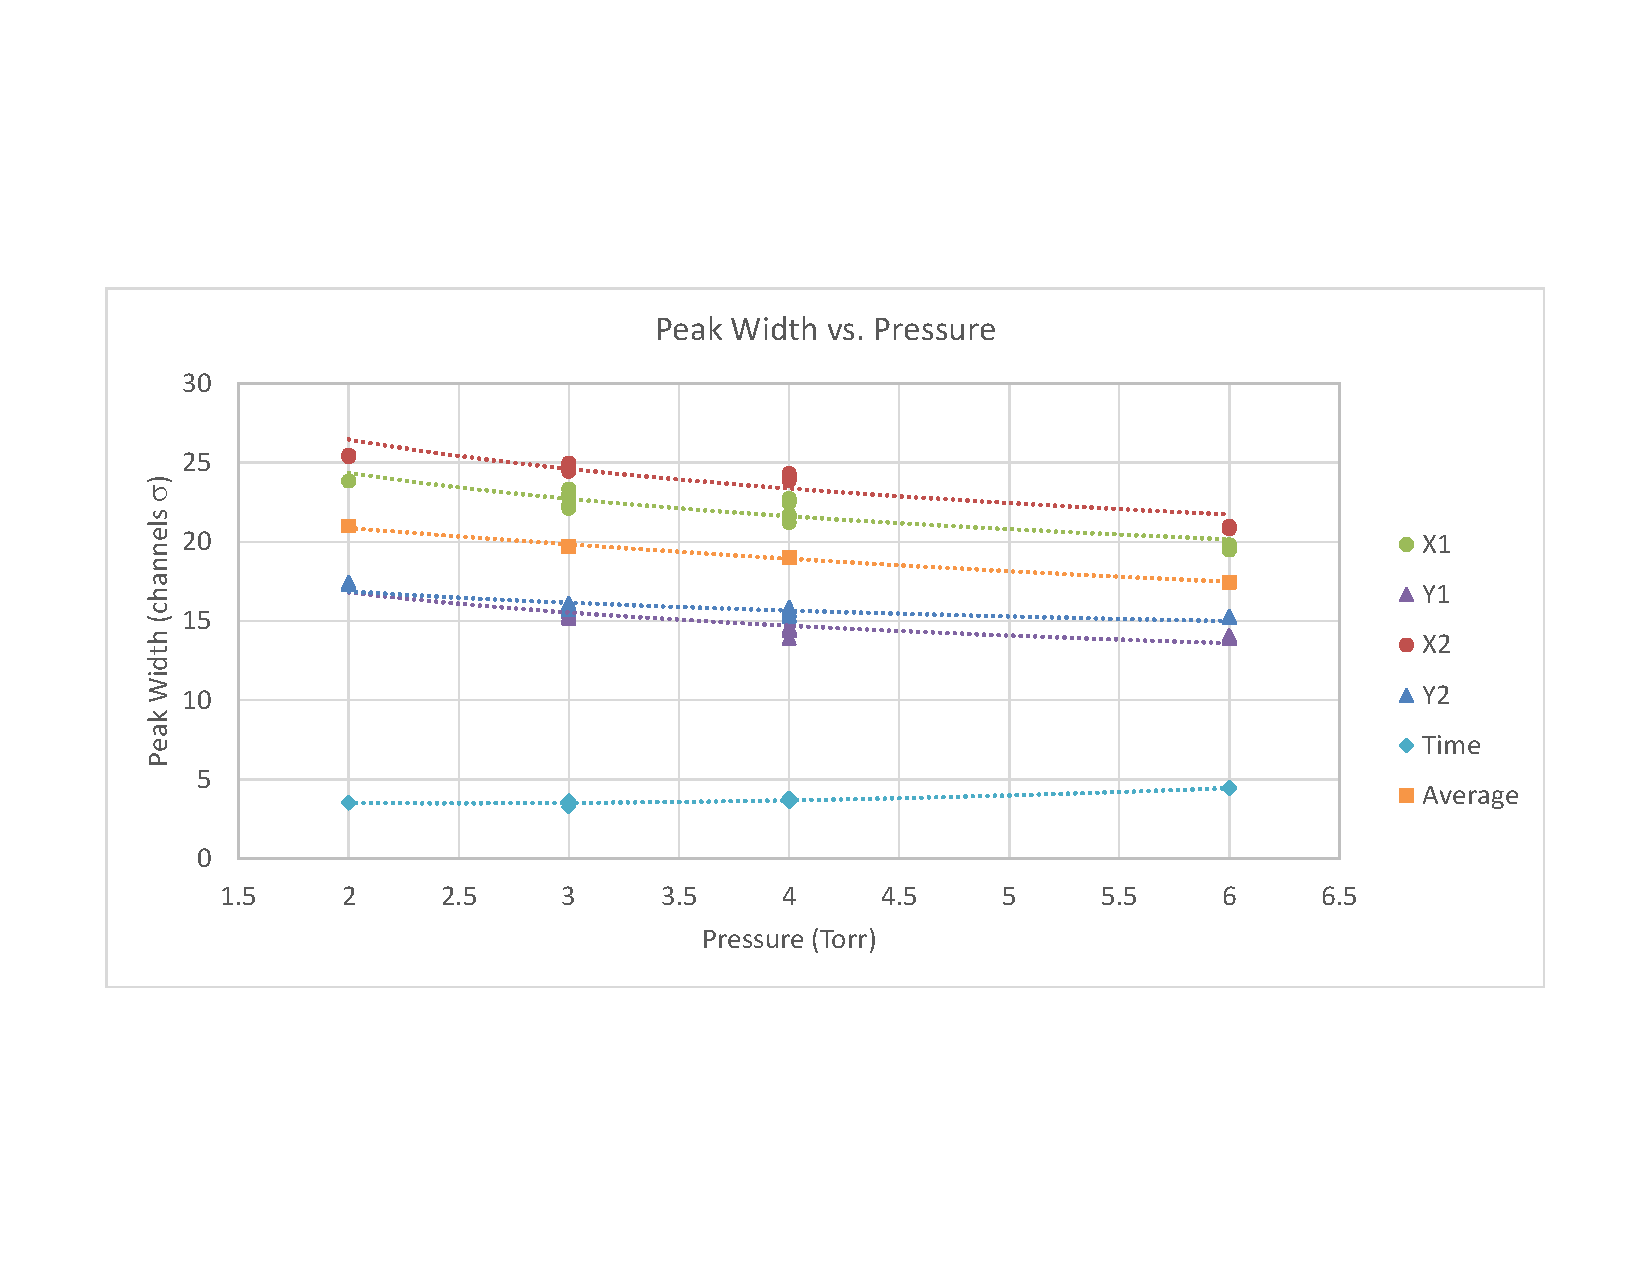
\includegraphics[width=\columnwidth, height=0.33\textheight, keepaspectratio]{PGAC_test_run_list_width_vs_P_6}%
\caption{Peak width variance with pressure. For each pressure setting, the detector is biased to the maximum stable operating voltage. The beam current was nominally 5.70\,enA for all runs. Each data set is fit with a quadratic function. The average of the positions is also plotted. These data are also given in Table~\ref{av_peak_vs_pressure}.}%
\label{pressure_width}%
\end{figure}

\begin{table}
\centering
\begin{tabular}{cccc|...}
\hline
& \multicolumn{3}{c}{Max Voltage} &\multicolumn{3}{c}{Average Peak Width}\\ \cline{2-4} \cline{2-4} \cline{5-7} 
$P$& $V_\textrm{c}$ & $V_\textrm{a}$ & $\Delta V$ &\multicolumn{1}{c}{Time}&\multicolumn{1}{c}{X}&\multicolumn{1}{c}{Y}\\
\hline \hline
2 & -80 & 395 & 475 & 3.54 & 24.64 & 17.39\\
3 & -75 & 410 & 485 & 3.50 & 23.72 & 15.68\\
4 & -80 & 430 & 510 & 3.69 & 23.06 & 14.98\\
6 & -90 & 450 & 540 & 4.46 & 20.27 & 14.64\\
\hline
\end{tabular}
\caption{Average peak width at the maximum stable operating voltage at each pressure. These data are plotted in Fig.~\ref{pressure_width}.}
\label{av_peak_vs_pressure}
\end{table}

\subsubsection{Position Dependence}
The output of the commands \texttt{peakfit()}, \texttt{peakfits()}, or \texttt{peakfity()}, in addition to providing linear position calibration, these commands will also output a plot of the individual peak widths. Given the global fit from which these parameters are generated, this is the most accurate procedure to assess the resolution of the detector. The width of the peaks shown in Fig.~\ref{peakfit} is shown in  Fig.~\ref{pos_width}.

\begin{figure}
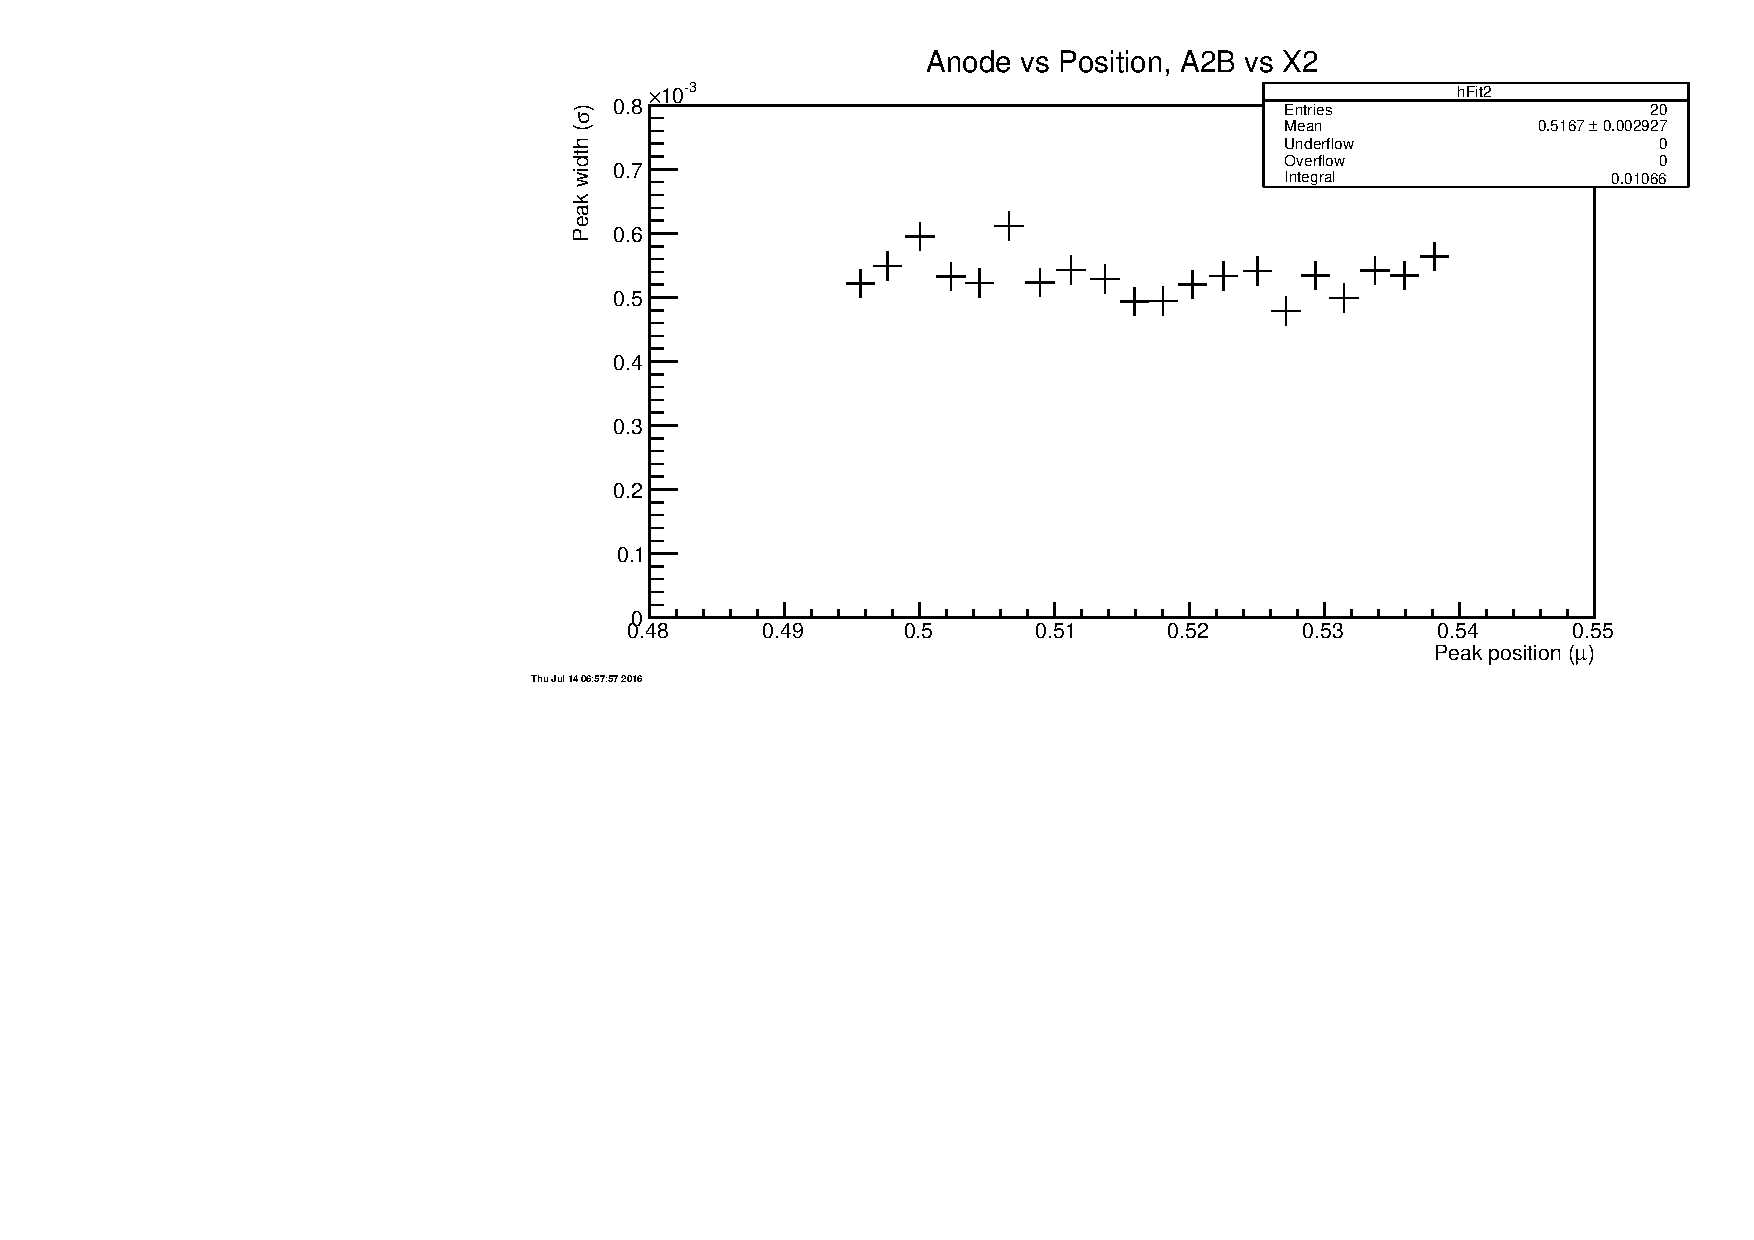
\includegraphics[width=\columnwidth, keepaspectratio]{run_606_width}%
\caption{Measured width of the peaks shown in Fig.~\ref{peakfit}. The widths are given in terms of the Gaussian fit parameter $\sigma$.}%
\label{pos_width}%
\end{figure}

\subsection{Timing Resolution}
The relationship between the anode signals was very sharply defined.  This allowed the anode signals to be gain-matched by applying a linear fit to a two-dimensional plot as shown in Fig.~\ref{lin_fit}.  
Equation~\ref{correlation} gives the relationship between the resolution 
%variance
 of the measured time $\sigma_{t}$ and the individual detector resolutions, $\sigma_{a1}$ and $\sigma_{a2}$.
\begin{equation}
\sigma_t^2=\sigma_{a1}^2+\sigma_{a2}^2-2\sigma_{a1}\sigma_{a2}
\label{correlation}
\end{equation}
Despite the clear correlation between the two anode signals (cf. Fig.~\ref{lin_fit}), the time measured by one anode does not effect the time measured by the other anode.  Therefore, in terms of the covariance of the two time measurements, the anode signals are uncorrelated.  This means that the last term in Eq.~\ref{correlation} is zero.  Assuming that the time resolution of both detectors is the same, Eq.~\ref{correlation} reduces to
\begin{equation}
  \sigma_{a}=\frac{1}{\sqrt{2}}\sigma_{t}.
\end{equation}

Therefore, to determine the timing resolution of an individual detector, the values of the timing resolution of the differences given in Tables~\ref{time_res} and \ref{time_res2} are divided by $\sqrt{2}$.
\paragraph{2014 Tests} 
For example, consider the width of the time difference  between the middle anode segments shown in Fig.~\ref{time_pos}; the width of the $y$-projection of the peak which is 2.23\,channels (sigma).  The TDC has a resolution of 200\,ps/channel.  Therefore the difference between the anode signals is calibrated to time in ns by dividing the channel number by 5.  In this case, the width of the difference corresponds to 446\,ps (sigma).  For an individual detector, this width is equivalent to 315\,ps (sigma) or 743\,ps~FWHM. The widths of the various time peaks is given in Table~\ref{time_res}.

\paragraph{2015 Tests} 
The timing resolution from the 2015 tests is given in Table~\ref{time_res2}.


\begin{figure}%
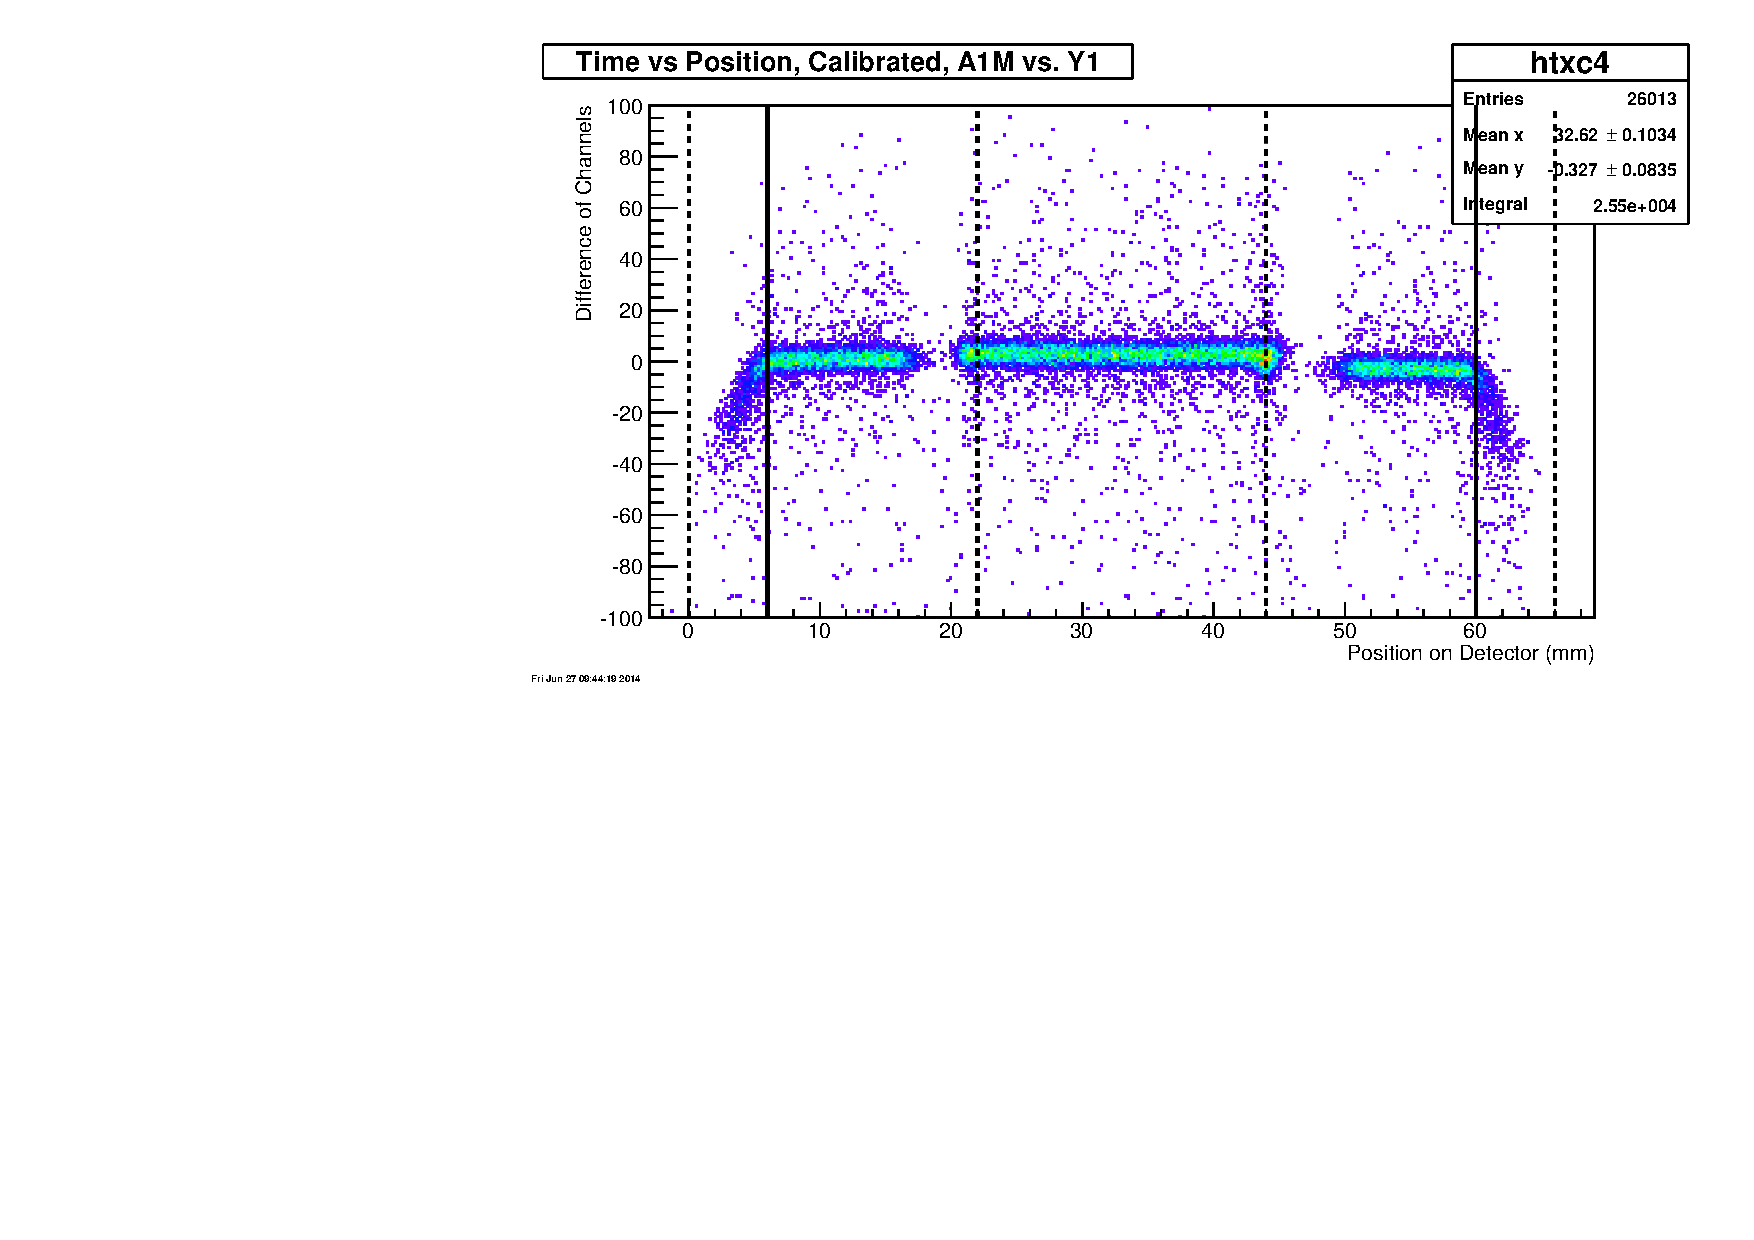
\includegraphics[width=\columnwidth]{run00480_htxc4}%
\caption{Plot of uncalibrated time vs. $y$-position on detector 1.  Solid lines indicate the positions of the Kapton shields.  Dashed lines indicate the edges of the anode segments.}%
\label{time_pos}%
\end{figure}
%\subsubsection{Results}
\begin{table}[ht!]
\centering
\begin{tabular}{-.....}
\hline
&\multicolumn{2}{c}{Pair}&&\multicolumn{2}{c}{Individual}\\ \cline{2-3} \cline{5-6}
\multicolumn{1}{c}{Reference}&\multicolumn{1}{c}{$\sigma$ (ns)}&\multicolumn{1}{c}{FWHM (ns)}&\multicolumn{1}{c}{$\mu$ (ns)}
                             &\multicolumn{1}{c}{$\sigma$ (ns)}&\multicolumn{1}{c}{FWHM (ns)}\\ \hline \hline
\textrm{A2}-\textrm{A1 (all)} & 0.6609 & 1.5563 & 0.0021 & 0.4673 & 1.1005\\
\textrm{A2B}-\textrm{A1B}     & 0.4730 & 1.1139 & -0.1616 & 0.3345 & 0.7877\\
\textrm{A2M}-\textrm{A1M}     & 0.4460 & 1.0502 & 0.2693 & 0.3154 & 0.7426\\
\textrm{A2T}-\textrm{A1T}     & 0.4656 & 1.0964 & -0.9179 & 0.3292 & 0.7753\\
%A2T-A1T (all)  & 0.6378 & 1.5019 & 0.4682\\
%\textrm{A2T}-\textrm{A1T (all)} & 0.6378&1.5019 &0.4682\\
\multicolumn{1}{c}{Average} & 0.4615 & 1.0868 & \multicolumn{1}{c}{---} & 0.3264 & 0.7685 \\
\hline
\end{tabular}
\caption{Timing resolution of the entire detector and the various anode segments. The timing between pairs of anode segments is given, excluding the overlap region near $x=44$\,mm. The equivalent timing resolution of an individual detector is also given (calculated by dividing by $\sqrt{2}$).
%\textit{<These values need to be updated; they are from before the anode signals were fully optimized and are little high.>}
}
\label{time_res}
\end{table}

\begin{table}[ht!]%
\centering
\begin{tabular}{-.....}
\hline
&\multicolumn{2}{c}{Pair}&&\multicolumn{2}{c}{Individual}\\ \cline{2-3} \cline{5-6}
\multicolumn{1}{c}{Reference}&\multicolumn{1}{c}{$\sigma$ (ns)}&\multicolumn{1}{c}{FWHM (ns)}&\multicolumn{1}{c}{$\mu$ (ns)}
                             &\multicolumn{1}{c}{$\sigma$ (ns)}&\multicolumn{1}{c}{FWHM (ns)}\\ \hline \hline
\textrm{A2B}-\textrm{A1B}   & 0.395 & 0.930 & 1.26 &0.279 & 0.658\\ 
\textrm{A2M}-\textrm{A1M}   &0.430 & 1.013 & -1.88 & 0.304 & 0.716\\ 
\textrm{A2T}-\textrm{A1T}   &0.369 & 0.868 & 0.53 & 0.261 & 0.614\\
\multicolumn{1}{c}{Average} & 0.398 & 0.937 &\multicolumn{1}{c}{---} & 0.281 & 0.663\\ \hline
\textrm{A2M}-\textrm{A1B}   & 0.928 & 2.185 & -44.41& 0.656 & 1.545\\ 
\textrm{A2B}-\textrm{A1M}   & 0.919 & 2.163 &-50.38 & 0.650 & 1.530\\ 
\textrm{A2M}-\textrm{A1T}   & 1.107 & 2.606 &-51.36 &0.783 & 1.843\\ 

\hline
\end{tabular}
\caption{Timing resolution of the various anode segments, given for Run 593. The timing between pairs of anode segments is given. The equivalent timing resolution of an individual detector is also given (calculated by dividing by $\sqrt{2}$).
%\textit{<These values need to be updated; they are from before the anode signals were fully optimized and are little high.>}
For reference, those pairs which have sharply-peaked time structure, but do not correspond to ``straight through'' trajectories, are also given.
}
\label{time_res2}
\end{table}

\subsection{Efficiency}
The left panel of Fig.~\ref{ruth} is similar to the final output from the \texttt{peakfit} commands. It shows the calculated area of each of the individual Gaussian fits using the equation
\begin{equation}
  \sigma\sqrt{2\pi} A.
\end{equation}
where $\sigma$ is the width of the fit and $A$ is the amplitude, given by the Gaussian fit parameters \texttt{0} and \texttt{2}, respectively. These values give an approximation of the number counts in the histogram attributable to each peak. The number of counts attributable to each peak would be directly related to the efficiency of the detector at the position of the peak if the detector was uniformly illuminated. However, the detector is not uniformly illuminated. The number of counts at each peak corresponds the Rutherford scattering cross section.

\begin{figure}
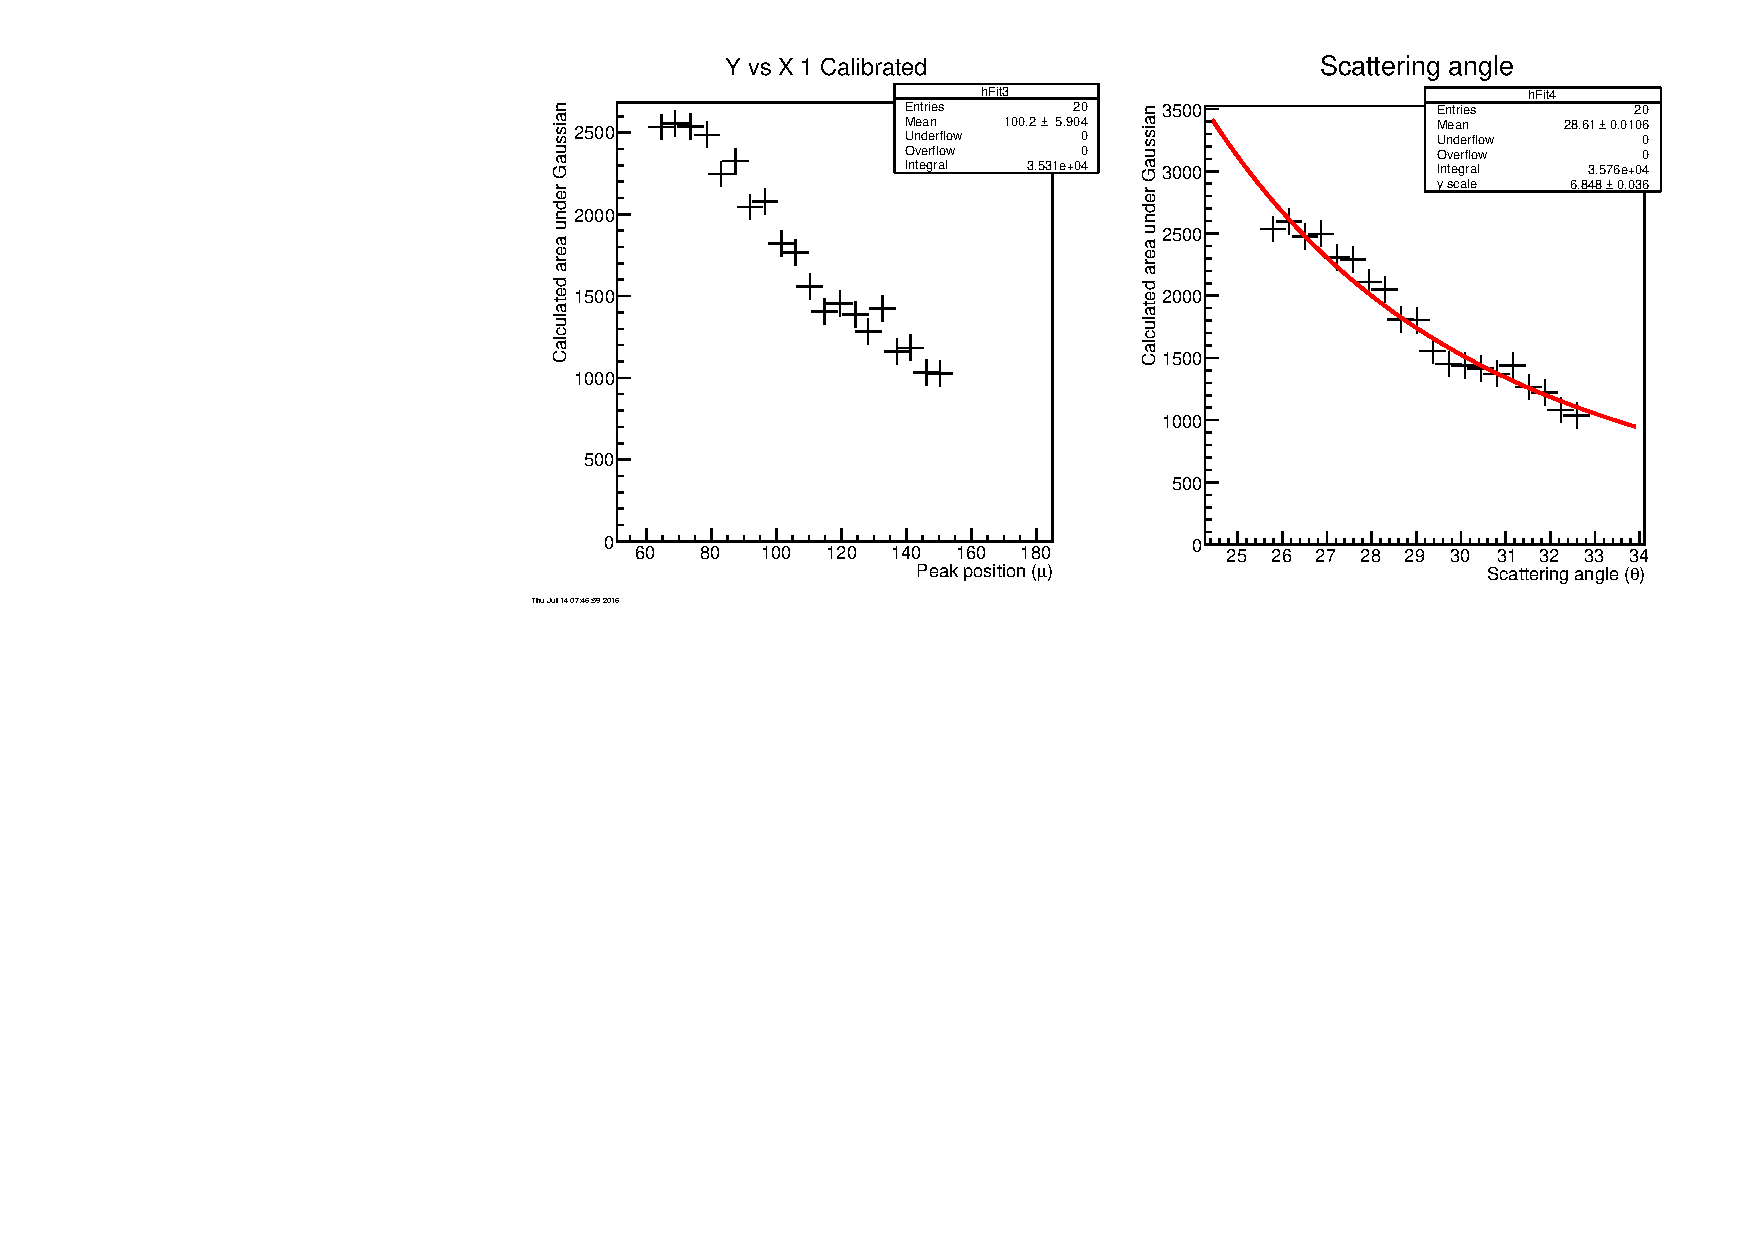
\includegraphics[width=\columnwidth, keepaspectratio]{run_606_ruth}%
\caption{}%
\label{ruth}%
\end{figure}

\begin{quote}
\begin{Verbatim}[firstnumber=0]
readandruth(0,3)
\end{Verbatim}
\end{quote}
The command \texttt{readandruth()} is an extension to the \texttt{peakfit} commands which includes the calculation of the Rutherford scattering cross section. The command takes as input two arguments. First, the detector number---\texttt{0} for detector 1 (downstream) and \texttt{1} for detector 2 (upstream). Right now only detector 1 is fully coded. The command makes a projection of the calibrated 2D position spectra---or ``hit patterns''---named \texttt{hhitc}. The second argument of the command gives the row number to measure, starting from the bottom of the detector. Calibration files are automatically read in so the position of the rows are known. After a particular row is selected, an $x$-projection is made thus giving the position spectrum for one row of peaks on the detector.

The normal peak-fitting routine is then run on the position spectrum. The final output of the peak-fitting routine, shown in the left panel of Fig.~\ref{ruth}, is the calculated area under the curve for each peak, given as a function of the calibrated detector position. The command \texttt{readandruth()} then performs a transformation of coordinates to calculate the scattering angle $\theta$ associated with each detector position. The information about the known height of the row provides the information needed to also calculate the azimuthal angle $\phi$. The plot on the right panel of Fig.~\ref{ruth} is generated, which shows the number of counts attributable to each peak as a function of calculated scattering angle. The distribution is then fit with a $\csc^4 (\theta/2)$ function where the amplitude of the function is a variable parameter. The relationship between the individual peak heights and the fit function may be used to gauge the position-dependence of the detector efficiency.